%!TEX root = ../thesis_a4.tex

\chapter[Impact of a tag recommendation system][Impact of a tag rec. system]{Impact of a tag recommendation system}
\label{sec:impact}

\section{Introduction}
\label{impact:sec:introduction}


%Online sharing platforms make extensive use of semantically-meaningful textual labels, called tags, to describe and annotate its contents. The use of these tags provides a means for searching, browsing and organising the resources of the platform. Systems that provide the functionality for making these annotations are normally referred to as collaborative tagging systems. In collaborative tagging systems, users of the online platform have the responsibility of annotating the content. Every relation between a tag and a content resource performed by a user of the system can be identified as a tag application~\cite{Sen}, and we refer to the set of all distinct tags that are assigned to a particular resource as a \textit{tagline}. The aggregate of all tag applications, which relate tags, resources and users of an online sharing platform, is normally known as the folksonomy~\cite{Wal2007Folksonomy}.

%In general, tags introduced using collaborative tagging systems are not restricted in its form, and users can freely create new tags at any time~\cite{marlow2006,Sen,Wagner2014}. This provides a great flexibility to collaborative tagging systems as opposed to other systems that make use of pre-defined vocabularies and that do not allow users to annotate content using non-existing terms in these vocabularies~\cite{Robu2009,Wagner2014}. Using such non-restricted vocabularies, users introduce new tags when the annotation of a particular resource requires it. Hence, they easily adapt to the evolution of the platform's content. Furthermore, it has been suggested that users feel more comfortable during the annotation process when they are not restricted to the use of a pre-defined vocabulary~\cite{Robu2009}. 

%Collaborative tagging systems suffer from a number of well-known problems including tag scarcity, the use of different tags to refer to a single concept (synonymy), the ambiguity in the meaning of certain tags (polysemy), typographical errors, the use of user-specific naming conventions, or the use of different languages~\cite{halpin2006}. It is often discussed whether the folksonomy of a collaborative tagging system, after a certain time of being in use, reaches a point of implicit consensus where the vocabulary converges to a certain set of tags and tagging conventions that are widely adopted by all users of the system~\cite{halpin2006,Sen,Sood2007,Robu2009,Wagner2014}. Such a consensus implies more coherent resource annotations and better opportunities for searching, browsing and content organisation~\cite{Spiteri2006}. Additionally, it leverages the value of the folksonomy as a source of knowledge mining~\cite{Wagner2014}. Some studies have analysed this aspect, and the emergence of consensus has been highlighted in several occasions~\cite{Robu2009,Wagner2014}. 

%According to these studies, the emergence of consensus depends on several factors, one of them being the way in which users are exposed to the annotations performed by other users. In general, the more users are exposed to the tagging conventions of other users, the fastest should the consensus emerge. In order to try to overcome some of the issues of collaborative tagging systems, tag recommendation systems can be employed to suggest potentially relevant tags during the annotation process of a resource~\cite{jaske2007}. These systems are generally based on the analysis of the content of the resources being annotated, or in the folksonomy of a collaborative tagging system. Former systems normally use feature extraction techniques to analyse content resources, and further training of machine learning models that can predict tags based on the extracted features (e.g.,~\cite{Li2006,turnbull2008,Toderici2010}). Folksonomy-based systems normally take advantage of tag co-occurrence information in previously annotated resources in order to provide relevant tag recommendations for newly annotated resources (e.g.,~\cite{Sigurbjornsson2008,Garg2008,DeMeo2009,ivanov2010,Font2013}).

%It can be intuitively hypothesized that a tag recommendation system, independently of its nature, should have an impact on the folksonomy of a collaborative tagging system. In fact, this has been suggested by many authors. \cite{golder2006} hypothesize that a tag recommendation system should help consolidating the tag vocabulary across users. The same idea is suggesed by J\"{a}schke et~al.~\cite{jaske2007} and Marlow et~al.~\cite{marlow2006}. J\"{a}schke et~al.~\cite{jaske2007,Jaschke2012} also hypothesize that tag recommendation should simplify the process of finding good tags for the resources being described and thus increase the chances of getting resources annotated.
%Similarly, Sood et~al.~\cite{Sood2007} hypothesize that by using a tag recommendation system, users can see how other users tag resources and better choose when to reuse already existing tags or when to create new ones. Therefore, tag recommendation should help alleviate synonymy problems and help vocabulary convergence~\cite{Sood2007}. These authors also hypothesize that the use of a tag recommendation system fundamentally changes the tagging process from being a generation process, where users must create tags from scratch, to being a recognition process, where users have to recognise valid tags from a list of suggestions. Zangerle et~al.~\cite{Zangerle2011} perform a study on \emph{hashtag} recommendation for Twitter\footnote{http://www.twitter.com}, a microblogging site, and hypothesize that the use of hashtag recommendation should help homogenising hashtags. Finally, Wang et~al.~\cite{Wang2012} hypothesize that tag recommendation can improve both the quality of tags and the efficiency of the tagging process, by clarifying the semantics of tags and reducing the manual cost of tagging.

In the previous chapters we have described a number of tag recommendation methods and evaluated them from different perspectives. In this chapter, we perform a large-scale experiment in which we analyse the impact of a tag recommendation system in the real-world folksonomy of Freesound. More specifically, we introduce the best performing recommendation method described in Chapter~\ref{sec:general} (RankP@$\percentageOfPercentageStrategy$, with$\percentageOfPercentageStrategy=0.15$) to the tagging system of Freesound with the classification extension described in Chapter~\ref{sec:class}, and analyse its impact on the site.

As we have seen in the literature review, many authors have hypothesised about the potential impact of tag recommendation in the folksonomies of online sharing sites (Sec.~\ref{sec:soa:impact_tag_recommendation}). Taking this into consideration, we can summarise the expected impact into the following three hypotheses:
\begin{enumerate}
\item \textit{Vocabulary convergence.} A tag recommendation system should contribute to the convergence and consolidation of a shared vocabulary across the users of a tagging system~\citep{golder2006,marlow2006,jaske2007,Sood2007,Zangerle2011}.
\item \textit{Quality of annotations.} A tag recommendation system should improve the quality of resource annotations in an online sharing platform~\citep{Naaman2008,Jaschke2012,Wang2012}.
\item \textit{Cost of the annotation process.} A tag recommendation system should reduce the cost of tagging, changing from a tag generation process to a tag recognition process~\citep{Sood2007,jaske2007,Wang2012}.
\end{enumerate}

Although there seems to be a consensus on the hypotheses, we are not aware of any study performing a deep analysis of the impact of a tag recommendation system into a real-world and large-scale folksonomy. Furthermore, even though several studies have focused on analysing aspects such as tagging behaviour or vocabulary convergence in tagging systems (Chapter~\ref{sec:SOA}), there is not a clearly defined set of evaluation metrics or methodology to carry out these analyses~\citep{farooq2007}.

In this chapter, we define a series of metrics to illustrate each of the three summarised hypotheses. Then, we compute the defined metrics for an extensive period of time comprising 2.5 years of Freesound analysis data, including three months after the introduction of tag recommendation. We put a special emphasis on analysing the changes observed before and after the introduction of tag recommendation. Our results give, for the first time, empirical and quantitative evidence of the validity of some of the previous hypotheses.
Specifically, our results show that tag recommendation effectively contributes to vocabulary convergence, partially contributes to an improvement of the annotation quality, but does not seem to significantly reduce the cost of the annotation process. 
%In closing, some suggestions are made regarding how could tag recommendation systems be improved to further increase the impact on some of the analysed aspects such as the quality of the annotations. 
Notice that both the definition of the metrics and the analysis of its results are relevant contributions of the present chapter.

The rest of this chapter is organised as follows. 
In Sec.~\ref{impact:sec:methodology}, we briefly summarise the components of the tag recommendation system that we implemented, and describe the evaluation metrics and analysis methodology. The results for all evaluated metrics, along with discussions about their implications, are reported in Sec.~\ref{impact:sec:results}. 
%In Sec.~\ref{impact:sec:discussion} we summarise our findings and discuss about the limitations of our analysis.
We end in Sec.~\ref{impact:sec:conclusion} with a discussion about our findings and future directions.


%%%%%%%%%%%%%%%%%%%%%%%%%%%%%%%%%%%%%%%%%%%%%%%%%%%%%%%%%%%%%%%%%%%%%%%%%%%%%%%%%%%%%%%%%%%%%%%%%%%%%%%%%%%%%
\section{Methods}
\label{impact:sec:methodology}


%%%%%%%%%%%%
\subsection{Tag recommendation algorithm}
\label{impact:sec:tag_recommendation_system}

As mentioned, the recommendation method implemented in the tagging system of Freesound corresponds to the class-based approach described in Chapter~\ref{sec:class}.
In summary, it is composed of the three main steps described in Chapter~\ref{sec:general} plus the class detection step added in Chapter~\ref{sec:class} (see Fig.~\ref{impact:fig:diagram}).
Given a set of input tags $\inputTags$, the recommendation method is able to generate several lists of candidate tags $\candidateTagsPerInputTag$ taking advantage of a tag-tag similarity matrix $\similarityMatrixOfClassH$ which is, in turn, derived from the analysis of a folksonomy $\folksonomy$. 
A particular similarity matrix $\similarityMatrixOfClassH$ is chosen after a class detection step in which the system predicts the audio class $\audioClass$ that better fits $\inputTags$.
%Several similarity matrices $\similarityMatrixOfClassH$ are precomputed which are tailored to particular audio classes $\audioClass$. 
%In the class detection step, the recommendation method can predict which audio class $\audioClass$ better fits $\inputTags$, and then use the corresponding similarity matrix. 
The different sets of candidates $\candidateTagsPerInputTag$ are then aggregated into a single set of tags with scores $\aggregatedCandidateTags$.
Finally, a simple heuristic is applied to decide which of the tags in $\aggregatedCandidateTags$ are relevant enough to form the set of recommended tags $\recommendedTags$ outputted by the recommendation method.

\begin{figure}
\centerline{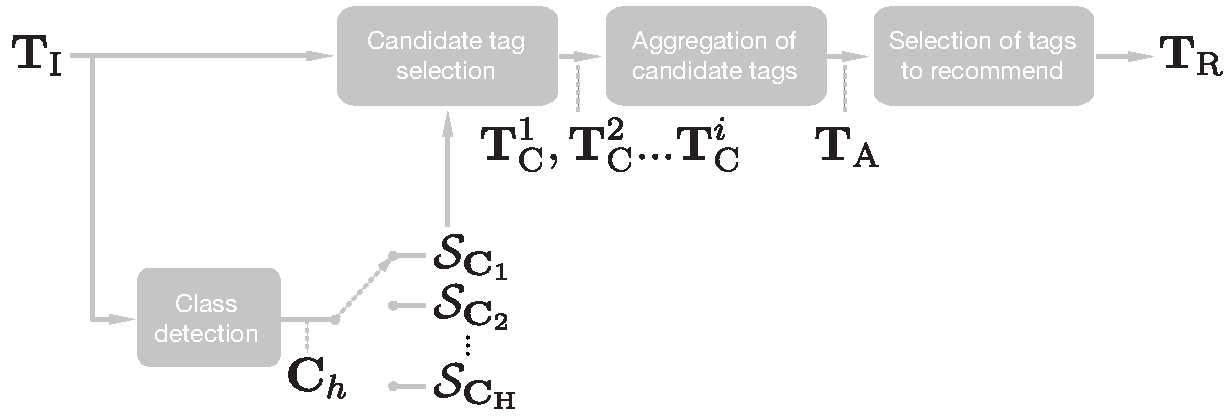
\includegraphics[width=\figSizeMidLarge]{ch05_impact/pics/fig01_diagram}}
\caption[Block diagram of the tag recommendation method implemented in Freesound]{Block diagram of the tag recommendation method implemented in the tagging system of Freesound.} 
\label{impact:fig:diagram}
\end{figure}

%\begin{enumerate}
%\item Class detection: The first step consists in the classification of the input tags $\inputTags$ into a set of $\nAudioClasses$ predefined audio classes. We defined $\nAudioClasses=5$ audio classes (\emph{SoundFX}, \emph{Soundscape}, \emph{Sample}, \emph{Music} and \emph{Speech}), and built a ground truth by manually annotating 1,200 Freesound sounds per class~\cite{Font2013a}. Using this ground truth, we trained a multivariate Bernoulli naive Bayes classifier, feeding it with the taglines of the sounds. Then, given a set of input tags $\inputTags$, the classifier can predict which category $\audioClass$ better fits the input.  Accuracies range between 75 and 95\%, depending on the length of $\inputTags$.

%\item Candidate tag selection: Given the set of input tags $\inputTags$, this step selects a pool of candidate tags $\candidateTagsPerInputTag$ for each input tag $\inputTag$. We do so by choosing the top 100 most similar tags according to a tag-tag similarity matrix $\similarityMatrix_{\audioClass}$, which depends on the predicted class $\audioClass$ of the previous step. Matrices $\similarityMatrix_{\audioClass}$ are computed offline and considering a model of the folksonomy of Freesound $\folksonomy$, which is represented as a tripartite hypergraph $\graph(\folksonomy)=\left\langle \vertices,\edges \right\rangle$~\cite{Mika2007a,Font2013}. In this model, vertices are given by three finite sets of objects, $\vertices=\users\cup \tags\cup \resources$ (users, tags and resources, respectively), and each edge $\edges=\{\{\user,\tagb,\resource\}| (\user,\tagb,\resource)$ $\in \folksonomy\}$ represents a tag application, embedding a relation between a tag $\tagb$, a resource $\resource$ (a sound), and the user $\user$ that performed that tag application. Given this model, we derive a sparse association matrix $\associationMatrix = \left\{ \associationMatrix_{i,j} \right\}$, $i=1,\dots |\resources|$, $j=1,\dots |\tags|$, which represents the associations between the $|\resources|$ sounds and the $|\tags|$ distinct tags available in Freesound ($\associationMatrixElement_{i,j} = 1$ if sound $\resource_i$ is labeled with tag $\tagb_j$, and $\associationMatrixElement_{i,j} = 0$ otherwise). 
%We use the same classifier used in the class detection step to predict the class of all sounds in the association matrix given their tag associations. Then, given $\associationMatrix$ and the list of sounds we predicted for every class $\audioClass$, we can compute the different tag-tag similarity matrices by filtering out all columns from $\associationMatrix$ corresponding to sounds which do not belong to a particular class and then performing a matrix multiplication so that $\similarityMatrix_{\audioClass} = \associationMatrixMultiplication'$, where $'$ indicates matrix transposition. Applying a simple normalisation to the elements of $\similarityMatrix_{\audioClass}$, we obtain a matrix whose elements $\left\{ \similarityMatrix_{\tagb_i,\tagb_j} \right\}$ correspond to the cosine similarity between tags $\tagb_i$ and $\tagb_j$ on the context of a particular audio class $\audioClass$~\cite{Font2013,Font2014}.

%\item Aggregation of candidate tags: Given the sets $\candidateTagsPerInputTag$ from the first step, candidates are assigned a score $\scoreCandidateTag$ and aggregated into a single list of tags with scores $\aggregatedCandidateTags$. Such score is determined by the candidate similarity-based ranking so that $\scoreCandidateTag=1$ for the most dissimilar candidate to a given input tag and $\scoreCandidateTag=N$ for the most similar one. The scores of tags that are present in different sets of candidates $\candidateTagsPerInputTag$ are added when aggregated to the final set $\aggregatedCandidateTags$~\cite{Font2013}.

%\item Selection of tags to recommend: Considering the scores in $\aggregatedCandidateTags$, this step determines a threshold $\scoreThreshold$ to select the tags that are finally recommended. The threshold $\scoreThreshold$ is set to be the 85\% of the maximum score in $\aggregatedCandidateTags$. Tags in $\aggregatedCandidateTags$ are sorted by their score and those that satisfy $\scoreCandidateTag \geq \scoreThreshold$ are outputted as $\recommendedTags$, the final set of recommended tags~\cite{Font2013}.
%\end{enumerate}

%%%%%%%%%%%%
\subsection{Tag recommendation interface}
\label{impact:sec:tag_rec_interface}

Fig.~\ref{impact:fig:screenshot_system} shows a screenshot of the interface for the tag recommendation system implemented in Freesound. In it, we can see the set of input tags $\inputTags=$\{\texttt{river}, \texttt{water}\} and the set of recommended tags $\recommendedTags=$\{\texttt{stream}, \texttt{creek}, \texttt{brook}, \texttt{flow}, \texttt{liquid}, \texttt{waterfall}, \texttt{trickle}\}. The list of suggested tags appears at the bottom of the text area that users use to type their tags, and it is automatically refreshed each time that users type a new tag (i.e.,~every time that there is a change in $\inputTags$). 
This means that during the annotation process of a particular sound, several lists of recommended tags are presented to the user. To introduce tags from the list of recommendations, users can either click on the elements of the list or type them manually (as they would do to introduce other tags that are not in the list). When manually typing tags, no autocomplete functionality is provided. 

\begin{figure}
\centerline{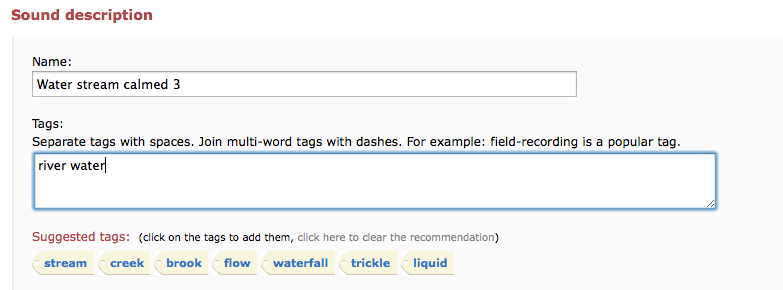
\includegraphics[width=1.0\columnwidth]{ch05_impact/pics/fig02_screenshot_system}}
\caption[Screenshot of the tagging interface of Freesound]{Screenshot of the tagging interface of Freesound after introducing the tag recommendation method. The previous interface (before the introduction of the tag recommendation), was exactly the same without the list of tag suggestions at the bottom.} 
\label{impact:fig:screenshot_system}
\end{figure}


%%%%%%%%%%%%
\subsection{Analysis metrics}
\label{impact:sec:definition_of_metrics}

To assess the impact that the tag recommendation system has on the folksonomy of Freesound, we define a series of metrics which are meant to illustrate the three hypotheses summarised in the introductory section of this chapter (Sec.~\ref{impact:sec:introduction}). 
Rather than the observation of a single metric being affected after the introduction of the tag recommendation system, we believe the relevance of the analysis particularly remains on the observation of changes simultaneously happening in several metrics. Hence, we illustrate each hypothesis with more than one metric.
Table~\ref{tab:hypothesis_metrics} shows a list of the defined metrics, along with the changes we expect to observe when comparing data before and after the introduction of the tag recommendation system. Formal metric definitions subsequently follow, grouped by hypothesis. 


\begin{table}
\ra{1.2}
\begin{center}
\footnotesize
	\begin{tabular}{p{3.7cm}P{4.8cm}P{3cm}}
	\toprule
	\textbf{Hypothesis} & \textbf{Metric} & \textbf{Expectation} \\
	\midrule
	\multirow{4}{3.7cm}{Vocabulary convergence}
	       & Percentage of new tags & Decrease \\
	 
	       & Average user vocabulary size & Increase \\ 
       	       & User vocabulary sharing & Increase \\ 
	       & Sound vocabulary sharing & Increase \\ 
	\\
	\multirow{5}{3.7cm}{Quality of annotations}
	       & Average tagline length & Increase  \\
	       & Percentage of misspelled tag applications & \multirow{2}{3cm}{Decrease}  \\ 
	       & Tag frequency distribution & Even (see caption)  \\ 
	       & Subjective annotation quality & Increase \\
	\\
	\multirow{3}{3.7cm}{Cost of the annotation process}
	       & Average tag application time & Decrease  \\
    	   & Average number of correctly predicted tags & \multirow{2}{3cm}{Similar to Sec.~\ref{class:sec:accepted_tags_results}}  \\
    \bottomrule
	\end{tabular}
\end{center}
\caption[Proposed metrics and expected observations]{Proposed metrics and expected observations to evaluate the hypotheses. In the case the tag frequency distribution, we expect a more even distribution across the frequency range after the introduction of tag recommendation.}
\label{tab:hypothesis_metrics}
\end{table}


\subsubsection{Vocabulary convergence}

\begin{itemize}
	\item \textit{Percentage of new tags}: This metric represents the percentage of the tag applications that were performed during a given day of our analysis period, and that had never been used before in the folksonomy (i.e.,~tag applications that introduce previously nonexistent tags in the folksonomy). Thus, this metric is computed on a daily basis (see Sec.~\ref{impact:sec:analysis_methodology}). Considering the folksonomy model defined in Sec.~\ref{sec:general:step1}, the percentage of new tags can be defined as
\begin{equation} \metricVocabularyConvergence(n) = 100 \cdot \frac{|\setOfNewTagsInDay|}{|\setOfTagApplicationsInADay|}, \label{impact:eq:percentage_of_new_tags} \end{equation}
where $\setOfNewTagsInDay$ is the set of tags that appeared for the first time in the $n$-th day of our analysis data, and $\setOfTagApplicationsInADay$ is the set of all tag applications performed during that same day. Note that $\setOfNewTagsInDay$ can not contain duplicates (i.e.,~a particular tag can not be considered as being ``new'' more than once). High values of $\metricVocabularyConvergence$ indicate that many new tags are being created and that, therefore, the vocabulary is not converging to a finite set of terms. Our expectation is that $\metricVocabularyConvergence$ will decrease after the introduction of tag recommendation, as users will tend to reuse tags from the list of suggestions rather than creating new ones.
		
	\item \textit{Average user vocabulary size}: This metric is also computed on a daily basis, and we define it as the total number of tag applications involving distinct tags that a user performed during a given day (i.e.,~the number of unique tags that a user assigned during a given day). Considering the folksonomy model defined in Sec.~\ref{sec:general:step1}, the average vocabulary size can thus be expressed as
\begin{equation} \metricAverageVocabularySize({n}) =  \frac{1}{|\setOfUsersPerformingTagApplicationInDay|}\sum\limits_{\user\in \setOfUsersPerformingTagApplicationInDay}{|\setOfTapplicationsDistinctTagsPerUserAndDay|}, \label{impact:eq:user_vocabulary_size} \end{equation}
where $\setOfTapplicationsDistinctTagsPerUserAndDay$ is the set of tag applications involving distinct tags that user $\user$ has performed during the $n$-th day of our analysis data, and $\setOfUsersPerformingTagApplicationInDay$ is the set of users that performed at least one tag application during that same day. High values of $\metricAverageVocabularySize$ indicate that users employ a wide variety of tags for annotating their sounds, whereas low values indicate that users tend to employ a restricted vocabulary of tags. We believe that when using the tag recommendation system users will be exposed to a wider variety of tags than the ones that they would have initially thought of. Hence, we expect to observe an $\metricAverageVocabularySize$ increase after the introduction of tag recommendation.

	\item \textit{User vocabulary sharing}: This metric quantifies to which extent users employ tags that have also been employed by other users. To analyse this aspect, we build a weighted network $\usersNetwork$ where nodes represent users and edges represent the amount of tags shared between two users. Edge weights $\edgeWeight$ between nodes $i$ and $j$ of $\usersNetwork$ are normalised using standard Jaccard similarity. Thus, given an arbitrary period of time $k$ for which a network $\usersNetwork_k$ can be constructed, the weight between two nodes can be computed as
\begin{equation}\edgeWeight_{ij} = \frac{ \left\vert \setOfDistincTagsPerUserAndPeriod \cap \setOfDistincTagsPerUserAndPeriodJ \right\vert }{ \left\vert \setOfDistincTagsPerUserAndPeriod \cup \setOfDistincTagsPerUserAndPeriodJ \right\vert }, \label{impact:eq:weight_vocabulary_sharing} \end{equation}
where $\setOfDistincTagsPerUserAndPeriod$ is the set of distinct tags that the user corresponding to the $i$-th node has annotated during the time period comprised in $k$ (similarly for $\setOfDistincTagsPerUserAndPeriodJ$ and node $j$). 
In such a network, two users will be strongly connected if they use the same tags when annotating their sounds. Notice that, according to the definition above, every node in $\usersNetwork_k$ has a self-loop, i.e.,~for $i=j$ we have $\edgeWeight_{i,j}=1$. Having defined $\usersNetwork_k$, node strength~\citep{Barrat2004} acts as a basic indicator of the level of vocabulary sharing across users. The more strength the nodes have, the more tags users are sharing. 
Let $\nNodes$ be the total number of nodes in $\usersNetwork_k$, and $\nodeStrength_i$ be the node strength for the $i$-th node of $\usersNetwork_k$ such that
\begin{equation} \nodeStrength_i = \sum\limits_{j=1}^{L}{w_{ij}}. \end{equation}
We define user vocabulary sharing $\metricUserVocabularySharing$ as the average node strength over the network so that
\begin{equation} \metricUserVocabularySharing(\usersNetwork_k) = \frac{1}{\nNodes}\sum\limits_{i=1}^{\nNodes}{\nodeStrength_i}. \label{impact:eq:user_vocabulary_sharing} \end{equation}

In our analysis, we build two networks $\usersNetwork_k$ as defined above, one considering all the data after the introduction of tag recommendation and the other considering data from a reference time window before the introduction of tag recommendation (see below). We compare these two networks by computing the difference between user vocabulary sharing (average node strength) in both networks. We asses the statistical significance of that comparison by taking the series of node strengths of both networks (i.e.,~without computing the average) and using the Kolmogorov-Smirnov two-sample test~\citep{Corder2009} for evaluating the null hypothesis that both node strength samples belong to the same distribution (we use a significance level of 0.01). After the introduction of tag recommendation, we expect to observe an increase in $\metricUserVocabularySharing$, as users will be highly exposed to the influence of tags used by other users, and therefore more links will be created in $\usersNetwork$.

	\item \textit{Sound vocabulary sharing}: Similar to the previous metric, we can also study the vocabulary sharing across sounds instead of users. In this way, sound vocabulary sharing represents the tags that sounds have in common. To analyse sound vocabulary sharing, we build a weighted network $\soundsNetwork$ where nodes represent sounds and edges represent the number of tags that are common in the two sounds linked by the edge. As in $\usersNetwork$, edge weights are normalised using the Jaccard similarity. Hence, the weight $\edgeWeight$ between nodes $i$ and $j$ of a network $\soundsNetwork_k$ computed with data from a time period $k$, can be defined as
\begin{equation} \edgeWeight_{ij} = \frac{ \left\vert \tagsAssignedToSoundI \cap \tagsAssignedToSoundJ \right\vert }{ \left\vert \tagsAssignedToSoundI \cup \tagsAssignedToSoundJ \right\vert }, \label{impact:eq:weight_sound_sharing} \end{equation}
where $\tagsAssignedToSoundI$ is the set of tags assigned to the sound represented by the $i$-th node (similarly for $\tagsAssignedToSoundJ$ and node $j$). Notice that, in this case, the definition of $\edgeWeight_{ij}$ does not include the time period $k$ in any of its terms. This is because all tag applications for a given sound are done at once. Therefore, if the sound was uploaded in the time period $k$ (and thus is represented by a node in the network $\soundsNetwork_k$), all its tag applications will have also been performed during that time period $k$. In $\soundsNetwork_k$, two sounds will be strongly connected if they are annotated with the same tags, and we consider node strength as a basic indicator of the vocabulary sharing across sounds. 
Thus, we can define sound vocabulary sharing $\metricSoundVocabularySharing$ for a network $\soundsNetwork_k$ as the average node strength over that network, and compute it in the same way as described for user vocabulary sharing.

%Therefore, we can define sound vocabulary sharing as the average node strength over a network $\soundsNetwork_k$ with $\nNodes$ nodes, so that
%\begin{equation} \metricSoundVocabularySharing(\soundsNetwork_k) = \frac{1}{\nNodes}\sum\limits_{i=1}^{\nNodes}{\sum\limits_{j=1}^{\nNodes}{\edgeWeight_{ij}}}. \label{impact:eq:sound_vocabulary_sharing} \end{equation}

For analysis purposes, we again build two networks with data before and after the introduction of tag recommendation. The two networks are compared in terms of their node strength following the same process described above for analysing user vocabulary sharing. After the introduction of tag recommendation, we expect to observe an increase in $\metricSoundVocabularySharing$, as users will be highly exposed to the influence of tags used by other users. Therefore, sound annotations will include these tags and more links will be created in the network $\soundsNetwork$.

\end{itemize}


\subsubsection{Quality of annotations}
\label{impact:sec:methods_quality_of_annotations}

\begin{itemize}

	\item \textit{Average tagline length}: This metric is computed on a daily basis, and we define it as the average number of tags assigned to sounds uploaded during a given day of our analysis period. Considering the folksonomy model defined in Sec.~\ref{sec:general:step1}, the average tagline length can be expressed as
\begin{equation} \metricAverageTaglineLength(n) =  \frac{1}{|\soundsUploadedInDay|}\sum\limits_{\resource\in \soundsUploadedInDay}{|\tagsOfSoundR|}, \label{impact:eq:average_tagline_length} \end{equation}
where $\tagsOfSoundR$ is the set of tags assigned to a resource $\resource$ and $\soundsUploadedInDay$ is the set of sounds uploaded and annotated during the $n$-th day of our analysis. High values of $\metricAverageTaglineLength$ indicate that sounds are being annotated with many tags, with potentially more comprehensive descriptions. Our expectation for this metric is to observe an increase after the introduction of tag recommendation, as the provided list of recommendations will help users to add more tags during the annotation process. In fact, even if recommendations are not appropriate, they may serve as a guide for users, and convey which kinds of information should be annotated about the sounds being described. For instance, the recommendation system could suggest a tag like \texttt{120bpm} to a sound sample corresponding to a music loop of different tempo. However, this tag might suggest to the user that she could describe tempo information, and help in this way to generate a longer tagline. %~\cite{Font2014}.
Hence, we expect $\metricAverageTaglineLength$ to be increased after the introduction of tag recommendation.


	\item \textit{Percentage of misspelled tag applications}: This metric represents the percentage of tag applications that contain tags with misspellings or typographical errors and that were performed during a given day of our analysis period. Considering the folksonomy model defined in Sec.~\ref{sec:general:step1}, the percentage of misspelled tag applications can be defined as
\begin{equation} \metricMispellings(n) = 100 \cdot \frac{|\setOfTagApplicationsInADayWithMisspellings|}{|\setOfTagApplicationsInADay|}, \end{equation}
where $\setOfTagApplicationsInADay$ is the set of all tag applications performed during the $n$-th day of our analysis data, and $\setOfTagApplicationsInADayWithMisspellings$ is the set of tag applications performed during that same day which involve misspelled tags.
In order to estimate $\setOfTagApplicationsInADayWithMisspellings$, we use a straightforward approach in which we check, for each individual tag, whether if it exists or not in an English dictionary. For that purpose we use the open-source Enchant spellchecking library, with British English and American English dictionaries\footnote{\url{http://www.abisource.com/projects/enchant/}.} \citep[similarly to][]{Guy2006}. 
We consider that the tags which do not appear in the English dictionary contain misspellings or typographical errors.
Using such a simple approach, tags consisting of proper nouns, compound words, or tags written in other languages, are most likely considered to be misspellings. However, we assume that the presence of these kind of tags is not affected by the introduction of the tag recommendation system, and thus our defined metric is meaningful enough for comparison purposes.
High values of $\metricMispellings$ indicate that many of the tags assigned to sounds contain misspellings. 
Our expectation is that $\metricMispellings$ should decrease after the introduction of tag recommendation, as users will manually type fewer tags and choose them from the list of recommendations instead.


	\item \textit{Tag frequency distribution}: One useful indicator of the impact of the tag recommendation system is the observation of changes in the frequency distribution of existing tags. 
Intuitively, tags that are very popular (i.e.,~that have a high frequency) tend to correspond to broader semantic concepts, while less popular tags usually correspond to narrower ones. Looking at the tag frequency distribution we can thus have an idea of users' tagging behaviour and observe if it is influenced by the tag recommendation system.
To do that, we compute the frequency of tags over a period of time $k$ such that the frequency $\tagFrequency$ of a tag $\tagb$ is expressed as
\begin{equation} \tagFrequency(\tagb,k) = |\tagApplicatonsPerTagT|, \label{impact:eq:tag_frequency} \end{equation}
where $\tagApplicatonsPerTagT$ is the set of all tag applications involving tag $\tagb$ during the time period $k$. We consider two time periods, one with data before the introduction of tag recommendation and the other with data after tag recommendation, and compute the complementary cumulative distribution of tag frequencies over the two periods. These kind of plots are common within the tagging literature~\citep{Bischoff2008,Robu2009}, and indicate the probability that the number of occurrences of a particular tag is above a certain level. By qualitatively comparing the resulting distribution over the two periods of time, we can have an idea of which frequency ranges are more affected by the tag recommendation system. We believe that the tag recommendation system will have a bigger impact on the tags with mid frequency of occurrence, in which the agreement in not as clear as in the tags with high frequencies. Therefore, our expectation for this metric is that we will observe a more even tag frequency distribution after the introduction of tag recommendation.

Additionally, we compare the distribution of tag frequencies before and after the introduction of tag recommendation in terms of their fit into a power law distribution. As mentioned, it has been suggested that folksonomies whose distribution of tag frequencies can be fitted by a power law exhibit mature vocabularies leading to better quality descriptions (Sec.~\ref{sec:soa:impact_tag_recommendation}). %~\citep{Mathes2004,Cattuto2006,halpin2006,Wagner2014}. 
Hence, we check if we observe any difference regarding this matter after the introduction of tag recommendation. %\ref{sec:soa:impact_tag_recommendation}
To check whether a distribution is well fitted by a power law we use the method proposed by~\cite{Clauset2007}\footnote{We use the open source implementation described in~\cite{Alstott2014}.}.
This analysis is also directly related with the hypothesis that tag recommendation should contribute to the convergence and consolidation of the vocabulary.

	\item \textit{Subjective annotation quality}: We are interested in analysing whether the tag recommendation system has an impact on the quality of sound annotations. To avoid having to define an objective metric for quality, we opt for measuring quality in relative terms, by comparing the subjective quality of a set of annotations before and after the introduction of tag recommendation. To do so, we set up a small online experiment where participants were presented with pairs of sounds from Freesound along with their taglines, and had to judge which sound was, in their opinion, better annotated. Every pair of sounds consisted of one sound uploaded after the introduction of tag recommendation and another sound uploaded before that. Sounds were labeled as ``Sound A'' and ``Sound B'', without providing any links to the original sounds in Freesound and without giving any hint of which sound was uploaded before and after the introduction of tag recommendation (Fig.~\ref{impact:fig:screenshot_experiment}). For every participant, sound pairs were presented in random order, and the assignment of each sound as being ``Sound A'' or ``Sound B'', was also randomised. For every pair of sounds, participants could either answer that ``Sound A'' was better annotated than ``Sound B'', that ``Sound B'' was better annotated than ``Sound A'', or indicate that they did not think that one sound was better annotated than the other (``No preference''). If participants wanted to give further explanations for their answers, they also had the option to introduce a textual comment for every comparison.
	
\begin{figure}
\centerline{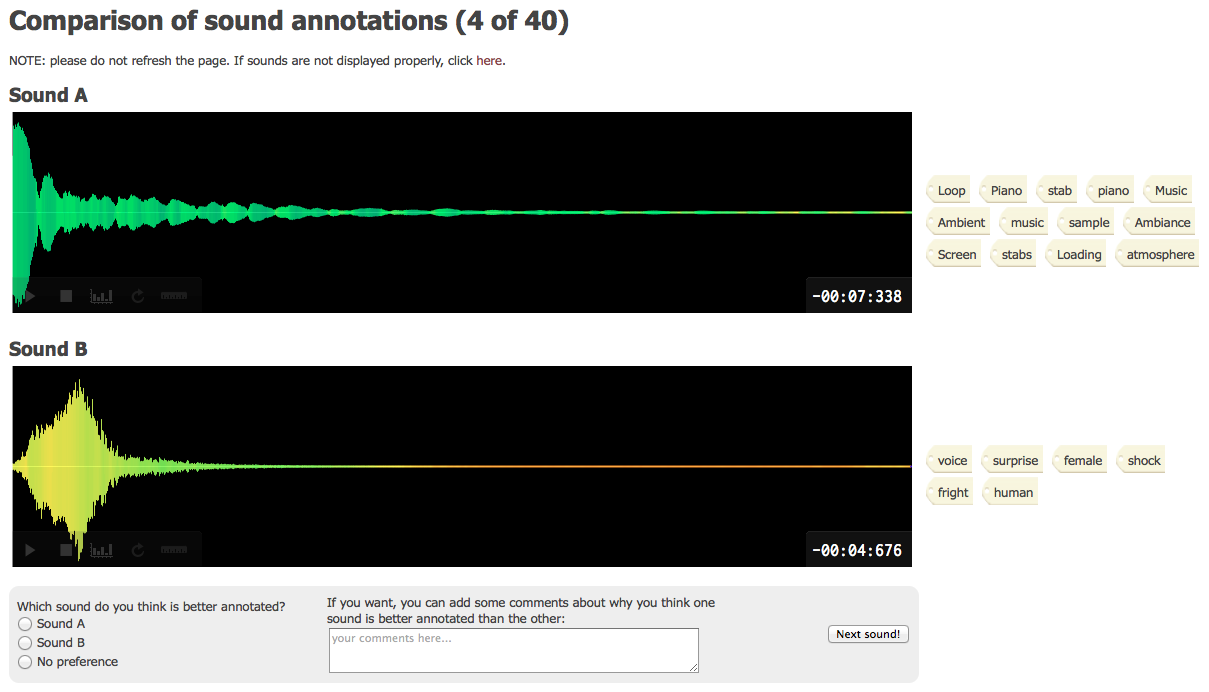
\includegraphics[width=1.00\columnwidth]{ch05_impact/pics/fig03_screenshot_experiment}}
\caption[Screenshot of the online experiment interface to judge the quality of annotations]{Screenshot of the online experiment interface to judge the quality of annotations.} 
\label{impact:fig:screenshot_experiment}
\end{figure}

Participants had to compare the annotation quality of a total of 40 sound pairs. To select the sounds for the experiment, we first randomly chose a set $\subjectiveEvaluationSetX$ of 40 sounds among those uploaded after the introduction of tag recommendation. The random selection was only constrained in such a way that all selected sounds had to be uploaded by different users. Then, we built another set $\subjectiveEvaluationSetY$ of 40 sounds uploaded before the introduction of tag recommendation. In order to build $\subjectiveEvaluationSetY$ and make it as similar as possible to $\subjectiveEvaluationSetX$ (i.e.,~containing similar kinds of recordings), we used the ``similarity search'' functionality of Freesound. For each sound $\subjectiveEvaluationSetX_i$, we retrieved a list of candidate similar sounds taking into account their acoustic properties represented by low-level audio descriptors\footnote{Low-level audio descriptors mainly include spectral features such as \emph{spectral centroid} and \emph{MFCC}. Note that the similarity search functionality does not take into account any metadata like tags or textual descriptions.}. Then, we pruned the lists of candidates by removing those sounds that were uploaded after the introduction of tag recommendation and by not allowing to have more than one sound uploaded by the same user. Finally, for each sound $\subjectiveEvaluationSetX_i$, we manually listened to the remaining candidates and selected the candidate that, in our opinion, was more acoustically similar to $\subjectiveEvaluationSetX_i$. %Set $\subjectiveEvaluationSetY$ was thus constructed with all  selected candidates. 
Having the sets $\subjectiveEvaluationSetX$ and $\subjectiveEvaluationSetY$, we formed the final pairs of sounds used in the experiment by iteratively selecting a random sound from each set until we got the 40 pairs determined. 

We asked the team of Freesound moderators\footnote{All sounds that are uploaded to Freesound are manually moderated by a small team of people (all of them long-term Freesound users) that ensure the appropriateness of the uploaded sounds. Hence, Freesound moderators are very familiarised with Freesound content and tagging particularities.} to participate in the experiment, and collected data from a total of seven participants (i.e.,~obtaining a total seven judgements for every sound pair). 	
Considering the collected data, we assign numerical values to the $i$-th quality judgement $\qualityJudgement_i$ performed by every participant such that
\begin{equation} \qualityJudgement_i = \begin{cases} 
	1 & \text{if } \subjectiveEvaluationSetX_i \text{ is better than } \subjectiveEvaluationSetY_i \\
	-1 & \text{if } \subjectiveEvaluationSetY_i \text{ is better than } \subjectiveEvaluationSetX_i \\
	0 & \text{if no preference.}
\end{cases} \label{impact:eq:quality_judgement_cases} \end{equation}
Then, qualitative annotation quality $\metricQualitativeAnnotationQuality$ is computed as the average over the union of all quality judgements $\qualityJudgement_i$ performed by all participants in the experiment. Let $\unionOfQualityJudgements$ be the union of all quality judgements $\qualityJudgement_i$. Then
\begin{equation} \metricQualitativeAnnotationQuality = \frac{1}{|\unionOfQualityJudgements|}\sum\limits_{j \in \unionOfQualityJudgements}{\unionOfQualityJudgements_j}. \label{impact:eq:quality_judgement_metric} \end{equation}
Note that a value of $\metricQualitativeAnnotationQuality$ close to $1$ indicates a preference for the annotations of sounds from $\subjectiveEvaluationSetX$ (i.e.,~sounds uploaded after the introduction of tag recommendation), while a value close to $-1$ indicates a preference for sounds from $\subjectiveEvaluationSetY$ (i.e.,~sounds uploaded before tag recommendation). A value close to $0$ indicates no preference. Our expectation for this metric is to obtain a positive value, indicating a tendency of considering sounds uploaded after tag recommendation as being better annotated than sounds uploaded before tag recommendation. This would suggest an increase in annotation quality.

\end{itemize}


\subsubsection{Cost of the annotation process}
\label{impact:sec:methods_cost_of_annotation}

\begin{itemize}

	\item \textit{Average tag application time}: An important indicator of how difficult it is for users to annotate sounds is the observation of the time they spend annotating them~\citep{Wang2012}. For that purpose, we define the average time per tag application as
\begin{equation} \metricAverageTagApplicationTime(\annotationSessions) =  \frac{1}{|\annotationSessions|}\sum\limits_{\annotationSession \in \annotationSessions}{\frac{\durationOfAnnotationSession}{|\tagApplicationsOfAnnotationSession|}}, \label{impact:eq:averae_tag_application_time} \end{equation}
where $\durationOfAnnotationSession$ is the duration of an annotation session $\annotationSession$ (in seconds), $\tagApplicationsOfAnnotationSession$ is the set of tag applications performed during an annotation session $\annotationSession$, and $\annotationSessions$ is a set of annotation sessions. Low $\metricAverageTagApplicationTime$ values indicate that users do not need much time to add a single tag, therefore it is presumably easy for them to describe sounds.

Unfortunately, Freesound did not log information about the duration of annotation sessions before the introduction of tag recommendation. Therefore, no data was available for most of the analysed time period. To overcome that issue, during a period of time that lasted two weeks between 24 March 2014 and 7 April 2014, we altered the tag recommendation system so that it only provided recommendations to half of the annotation sessions (but logged the annotation process in both cases). Therefore, our analysis of $\metricAverageTagApplicationTime$ is carried out with data gathered only during that extra analysis period. This data includes annotation sessions for 562 sounds, one half of them annotated using tag recommendation and the other half annotated without tag recommendation. Note that this new analysis period does not overlap with the period of the main analysis (see below).

We divide the annotation session data we gathered into two sets: one containing data from sessions were tag recommendations were not provided ($\annotationSessions^-$) and the other containing data from sessions with recommendations ($\annotationSessions^+$). Next, we compare the average $\metricAverageTagApplicationTime$ for both sets of annotation sessions and asses the statistical significance of the difference by performing the Mann-Whitney U test with a significance level of 0.01~\citep{Corder2009}. Our expectation for this metric is that sessions which provided tag recommendations will exhibit lower values of $\metricAverageTagApplicationTime$, as users will add some tags by clicking on the tag suggestions and this will make the annotation process faster.

	\item \textit{Average number of correctly predicted tags}: This is the main metric that we used in the user-based evaluation carried out in the previous chapter (Sec.~\ref{class:sec:evaluation}). It quantifies how many of the tags assigned to a sound during an annotation process were actually suggested by the recommendation system (thus correctly predicted). We follow the definition of Eq.~\ref{class:eq:n_accepted_tags}. However, here we define it on a daily basis such that
\begin{equation} 
%\metricPercentageOfCorrectlyPredictedTags(n) = \frac{1}{|\soundsUploadedInDay|}\sum\limits_{\resource\in \soundsUploadedInDay}{| \tagsOfSoundR \cap \setOfTagsSuggestedToSoundR |},
\nAcceptedTags(n) = \frac{1}{|\soundsUploadedInDay|} \sum\limits_{\resource\in \soundsUploadedInDay}{\left\vert \tagsOfSoundR \cap \left( \bigcup^{\numberOfTagRecommendationsInSession}_{\recommendationsInSessionIndex=1} \nthRecommendedTagsInSession \right) \right\vert}, 
\label{impact:eq:percentage_of_correctly_predicted_tags} \end{equation}
where $\tagsOfSoundR$ is the set of tags assigned to sound $\resource$, 
$\nthRecommendedTagsInSession$ is one of the sets of recommended tags that were presented to the user in the successive $\numberOfTagRecommendationsInSession$ recommendations during the tagging process of $\resource$, and $\soundsUploadedInDay$ is the set of sounds uploaded and annotated during the $n$-th day of our analysis data. Note that we can not compute $\metricPercentageOfCorrectlyPredictedTags$ for data before the introduction of tag recommendation. 

The average number of correctly predicted tags is an indicator of the usefulness of the tag recommendation system during the annotation process. High values of $\metricPercentageOfCorrectlyPredictedTags$ indicate that many of the tags that are recommended are actually used to annotate the sounds they are recommended for, and suggest that the annotation process is less costly as tags are taken from the list of suggestions. Our expectation for this metric is to obtain similar results as in the user-based evaluation of Chapter~\ref{sec:class} (Table ~\ref{tab:results_general_ub}). %In that case, the average number of correctly predicted tags was found to be 2.414 for the class-based tag recommendation method (Table ~\ref{tab:results_general_ub}).


\end{itemize}


%%%%%%%%%%%%
\subsection{Analysis methodology}
\label{impact:sec:analysis_methodology}

The impact of the tag recommendation system is analysed by looking at the evolution of the Freesound folksonomy (gathering data directly from the Freesound database) and the logs we create every time a user annotates a new sound. Our analysis comprises data between the 21 September 2011 and 28 February 2014. The tag recommendation system was introduced on 20 November 2013. The metrics defined in the previous section are either computed on a daily basis (using data from a particular day of our analysis), or over bigger periods of time (using data data gathered from several days of our analysis). To represent daily time periods, let $\mathbf{\daysVector}$ be a vector of time periods where $\daysVector_{n}$ corresponds to the time period of the $n$-th day since the beginning of our analysis data. In that vector, $\daysVector_{0}$ corresponds to the time period of the first day in our analysis data (21 September 2011), and $\daysVector_{N}$ corresponds to the time period of the last day for which we have analysis data (28 February 2014). 

In addition to what precedes, to represent larger periods of time, we define a series of analysis windows which include data from several days of our analysis. On the one hand, let $\windowOfInterest$ be our analysis window of interest, which represents a time period including all the data after the introduction of tag recommendation (i.e.,~a total of 100 days from 20 November 2013 to 28 February 2014). On the other hand, let $\referenceWindowsVector$ be a vector of reference analysis windows where each element $\referenceWindowsVector_{m}$ corresponds to a time period of the same length as $\windowOfInterest$ (100 days), drawn from data before the introduction of tag recommendation. The window $\referenceWindowsVector_{0}$ corresponds to the last 100 days before the introduction of tag recommendation (from the 12 August 2013, to 19 November 2013), and the $m$-th analysis window corresponds to a time period shifted backwards in time $50m$ days. Figure~\ref{impact:fig:analysis_windows} shows a graphical representation of $\mathbf{\daysVector}$ and $\referenceWindowsVector$, and the analysis window of interest $\windowOfInterest$. Notice that $\windowOfInterest$, as well as each element of $\referenceWindowsVector$, includes a particular range of $\daysVector$ time periods (e.g.,~$\windowOfInterest$ corresponds to $\daysVector_{N-100:N}$).

\begin{figure}
\centerline{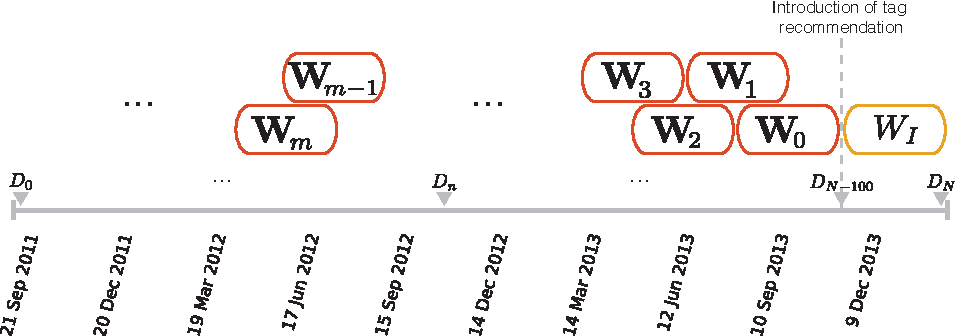
\includegraphics[width=1.0\columnwidth]{ch05_impact/pics/fig04_analysis_windows}}
\caption[Time period vectors and analysis windows]{Time period vectors $\daysVector$ and $\referenceWindowsVector$, and the analysis window of interest $\windowOfInterest$.}
\label{impact:fig:analysis_windows}
\end{figure}

As mentioned, we are interested in comparing the results of the defined metrics for time periods \emph{before} and \emph{after} the introduction of tag recommendation. In the case of metrics that are computed on a daily basis, we perform the comparison by computing the average of each metric over the range of days in $\mathbf{\daysVector}$ included in the window of interest $\windowOfInterest$ and in each reference window $\referenceWindowsVector_{m}$. Then, the average obtained from $\windowOfInterest$ is compared with the average obtained for each time period $\referenceWindowsVector_{m}$. This results in a total of $M$ comparisons per metric. In our results section, and unless stated otherwise, we always report the results of the comparison between $\windowOfInterest$ and the $\referenceWindowsVector_{m}$ that yields the minimum difference. Hence, our results only show the case in which the tag recommendation system has the least impact. For each one of these comparisons, we assess statistical significance by taking the daily results of the metric corresponding to the compared time periods $\windowOfInterest$ and $\referenceWindowsVector_{m}$ and performing the Mann-Whitney U test with a significance level of 0.01. For the case of metrics that are not computed on a daily basis, we follow different approaches for comparing and assessing statistical significance. These approaches  have been described for every particular metric in corresponding subsections of Sec.~\ref{impact:sec:definition_of_metrics}.

Our analysis data includes annotations for sounds of very different natures and from users with very different levels of expertise. During the analysis period, some users uploaded only one sound, while others uploaded thousands, with the average being on 12.7 uploaded sounds per user. % min:1, max:5655, avg: 12.69, med: 2, 75th perc: 7
A final point to note is that, although we do not perform any cleaning of the considered Freesound data, we remove from our consideration all tag applications performed by a specific user that, during a narrow time period within $\windowOfInterest$ (from 17 January 2014 to 27 January 2014), intensively uploaded and annotated sounds using three times more tags per sound than the average. We considered this user as being a clear outlier that could potentially bias the results of our analysis magnifying the observed impact of tag recommendation. %by significantly increasing the average tagline length after the introduction of tag recommendation.


%%%%%%%%%%%%%%%%%%%%%%%%%%%%%%%%%%%%%%%%%%%%%%%%%%%%%%%%%%%%%%%%%%%%%%%%%%%%%%%%%%%%%%%%%%%%%%%%%%%%%%%%%%%%%
\section{Results and discussion}
\label{impact:sec:results}


%%%%%%%%%%%%
\subsection{Vocabulary convergence}
\label{impact:sec:results_vocabulary_convergence}


\subsubsection{Percentage of new tags}
\label{impact:sec:percentage_of_new_tags_results}

\begin{figure}
\centerline{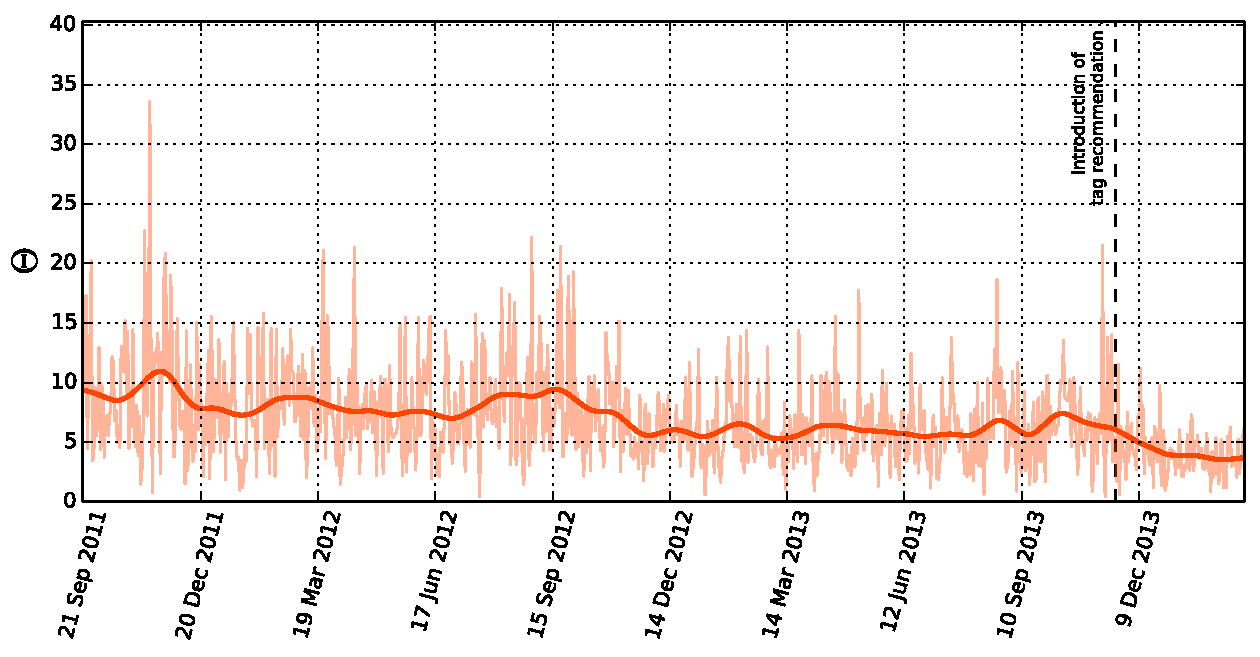
\includegraphics[width=\figSizeMax]{ch05_impact/pics/fig05_percentage_new_tags}}
\caption[Evolution of the percentage of new tags]{Evolution of the percentage of new tags $\metricVocabularyConvergence$. The thinner line corresponds to computed $\metricVocabularyConvergence$. The bold line corresponds to a smoothed version of $\metricVocabularyConvergence$. Smoothing is performed by convolution over a moving Hann window of 51 days. That particular number of days has been arbitrarily chosen to generate an informative yet visually appealing figure. Unless stated otherwise, the same smoothing strategy is applied in the other figures in this chapter.} 
\label{impact:fig:percentage_new_tags}
\end{figure}

Fig.~\ref{impact:fig:percentage_new_tags} shows the evolution of the percentage of new tags $\metricVocabularyConvergence$ over the considered time period. We see that, as expected, it qualitatively decreases after the introduction of tag recommendation. The minimum difference we observe between $\windowOfInterest$ and all $\referenceWindowsVector_m$ is a decrease of 1.7\%, which is found to be statistically significant ($\pvalue = 4.01\cdot 10^{-6}$). The maximum difference we observe is a decrease of 5\% ($\pvalue = 1.26 \cdot 10^{-15}$). 

The depicted evolution suggests an influence of the tag recommendation system on the percentage of new tags. However, looking at Fig.~\ref{impact:fig:percentage_new_tags}, a decreasing global trend can be qualitatively observed, even before the introduction of tag recommendation.
To compensate for the existence of such a trend, we perform an extra analysis in which we apply a correction to the $\metricVocabularyConvergence$ data points obtained from $\windowOfInterest$. The correction consists in computing a linear regression with all data points before the introduction of tag recommendation and then subtracting the linear projection of that trend to the data after the introduction of tag recommendation. Once we apply the correction to $\metricVocabularyConvergence$ over the window $\windowOfInterest$, we repeat the comparisons with all reference windows $\referenceWindowsVector_m$ and observe, this time, a minimum $\metricVocabularyConvergence$ decrease of 1.5\% which still remains statistically significant ($\pvalue = 5.68\cdot 10^{-5}$).
The observed global decreasing trend might be explained by a vocabulary consolidation process inherent to the tagging system, which is later accelerated with the introduction of tag recommendation.

It could be further argued that during the time period between 15 September 2012 and 14 December 2012 a localised decreasing pattern can also be observed with a similar strength to the one we observe after the introduction of tag recommendation. 
This decreasing pattern might be explained by the apparent local increase that can be observed in the previous months, which might be provoked by a particular user uploading a significant number of sounds with many new tags. Importantly, no relevant patterns can be observed in the other studied metrics during that particular period of time (see below). Moreover, just by simple observation of Fig.~\ref{impact:fig:percentage_new_tags}, it can be spotted that the variance of $\metricVocabularyConvergence$ is smaller after the introduction of tag recommendation, thus giving more relevance to the observed decreasing pattern during $\windowOfInterest$. 
As mentioned, it is the consideration of similar results from several different metrics that allows us to draw conclusions regarding the formulated hypotheses. 




\subsubsection{Average user vocabulary size}
Fig.~\ref{impact:fig:user_vocabulary_size} shows the evolution of the average user vocabulary size $\metricAverageVocabularySize$. In it, a clear impact of the tag recommendation system can be observed, as $\metricAverageVocabularySize$ consistently increases after the introduction of tag recommendation. When comparing results for the analysis window $\windowOfInterest$ and the other reference windows $\referenceWindowsVector_m$, we found a minimum $\metricAverageVocabularySize$ increase of 3.46 tags per user ($\pvalue = 2.303\cdot 10^{-11}$). 
This demonstrates that, after the introduction of tag recommendation, users tend to use a wider variety of tags as their vocabulary size is significantly increased.


\begin{figure}
\centerline{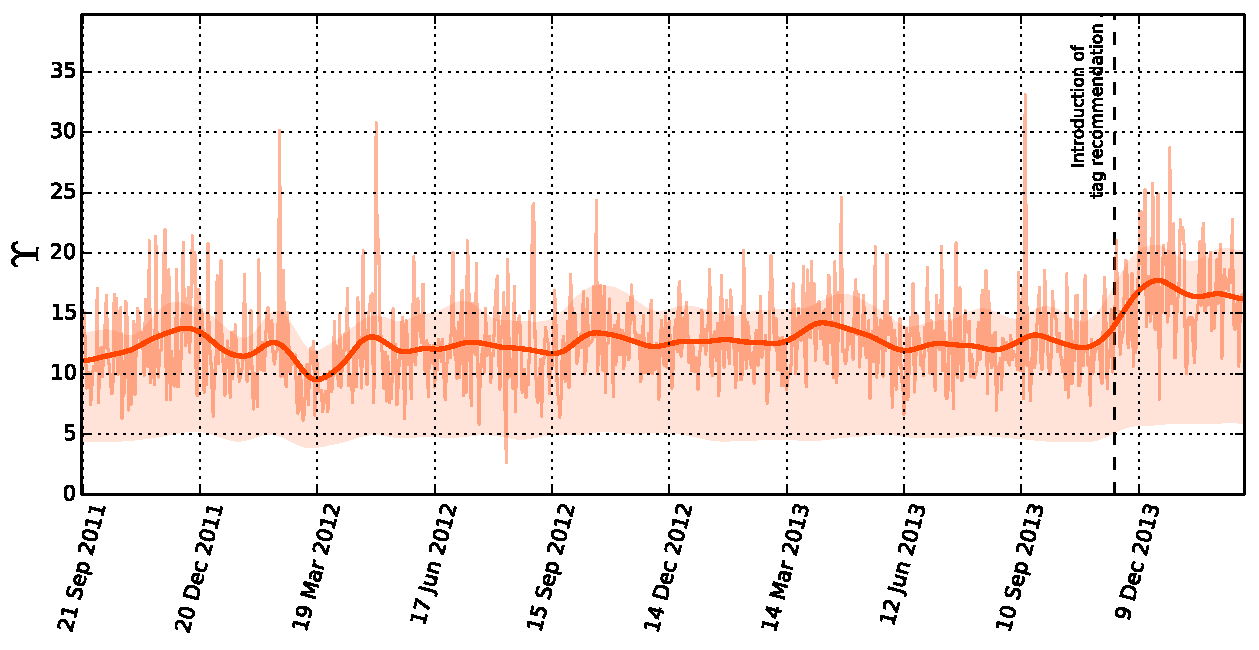
\includegraphics[width=\figSizeMax]{ch05_impact/pics/fig06_user_vocabulary_size}}
\caption[Evolution of average user vocabulary size]{Evolution of average user vocabulary size $\metricAverageVocabularySize$. The thinner line corresponds to computed $\metricAverageVocabularySize$. The bold line corresponds to a smoothed version of $\metricAverageVocabularySize$. The filled area shows the range between the lower and upper quartiles of the original data. 
}
\label{impact:fig:user_vocabulary_size}
\end{figure}


\subsubsection{User vocabulary sharing}
\label{impact:sec:vocabulary_sharing_users}
% 73240/1148 = 63.79
% 122474/1335 = 91.74
As described in Sec.~\ref{impact:sec:definition_of_metrics}, to analyse user vocabulary sharing ($\metricUserVocabularySharing$) we built two networks using data before and after the introduction of tag recommendation.
In particular, we use data from the analysis windows $\referenceWindowsVector_0$ and $\windowOfInterest$, respectively. The resulting network built with data from $\referenceWindowsVector_0$ has a total of 1,148 nodes (i.e.,~users) and 73,240 edges (yielding a ratio of 63.79 edges per node), whereas the network built with data from $\windowOfInterest$ features 1,335 nodes and 122,474 edges (91.74 edges per node). Just by looking at these numbers, it can already be seen that users in the $\windowOfInterest$ network are much more connected among them. Fig.~\ref{impact:fig:users_graph_strength} shows the complementary cumulative node strength distribution of the two networks. The distribution shows that, for a given probability, the network after the introduction of tag recommendation features nodes with a higher strength. Comparing the two distributions yields a statistically significant $\metricUserVocabularySharing$ increase of 2.12 ($\pvalue = 8.652\cdot 10^{-17}$). 
These observations highlight that the tag recommendation system effectively favours tags sharing among users. 

\begin{figure}
\centerline{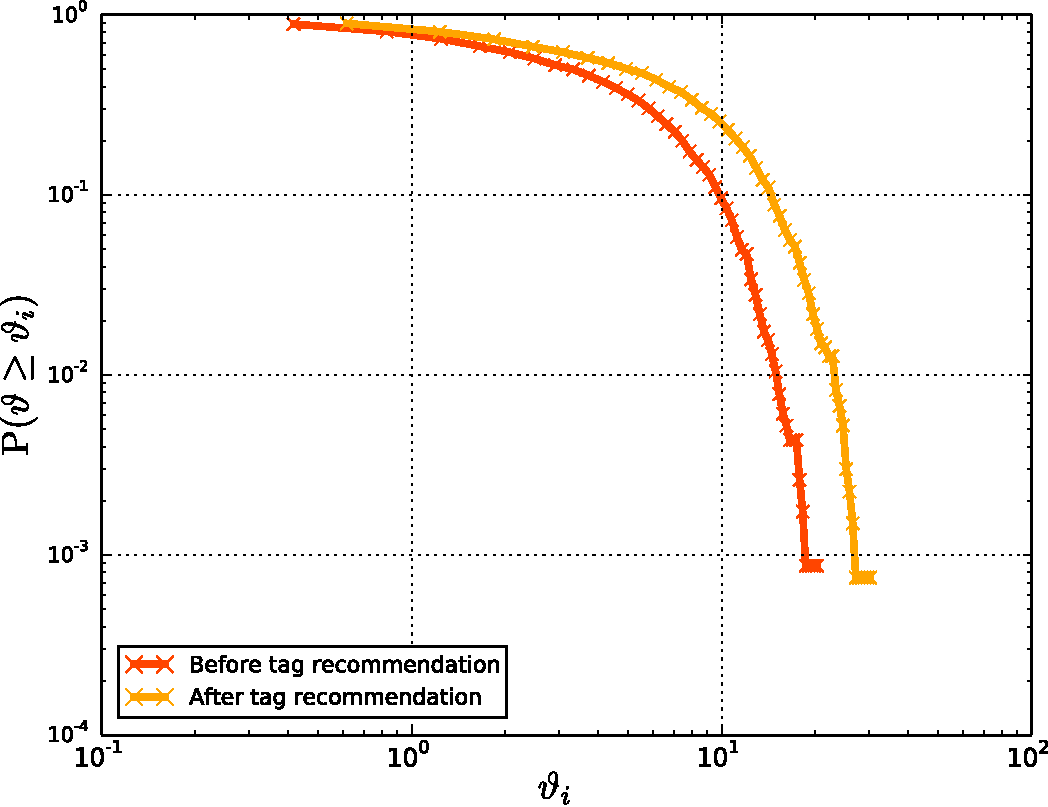
\includegraphics[width=0.66\columnwidth]{ch05_impact/pics/fig07_users_graph_strength}}
\caption[Complementary cumulative node strength distribution of user-user network]{
Complementary cumulative node strength $\nodeStrength$ distribution of user-user network $\usersNetwork$ before and after the introduction of tag recommendation. Networks are build with data from analysis windows $\referenceWindowsVector_0$ and $\windowOfInterest$ respectively.}
\label{impact:fig:users_graph_strength}
\end{figure}


\subsubsection{Sound vocabulary sharing}
% 3414449/9898 = 344.97 abans
% 7405037/12946 = 571.99 dps
The analysis of sound vocabulary sharing $\metricSoundVocabularySharing$ reports similar results to those of user vocabulary sharing. The resulting network built with data from $\referenceWindowsVector_0$ has a total of 9,898 nodes (i.e.,~sounds) and 3,414,449 edges (yielding a ratio of 344.97 edges per node), whereas the network built with data from $\windowOfInterest$ features 12,946 nodes and 7,405,037 edges (571.99 edges per node). Again, it can already be observed that the network after tag recommendation is much more connected. Fig.~\ref{impact:fig:sounds_graph_strength} shows the complementary cumulative node strength distribution of the two networks. In this case, we also observe an statistically significant overall increase of node strengths after the introduction of tag recommendation. Interestingly, this is somewhat more relevant in the range of sounds that used to be less connected in the network (roughly for $\nodeStrength < 200$). The average $\metricSoundVocabularySharing$ increase is of 34.26 ($\pvalue = 2.606\cdot 10^{-231}$). This result is consistent with what we find in the case of user vocabulary sharing.

\begin{figure}
\centerline{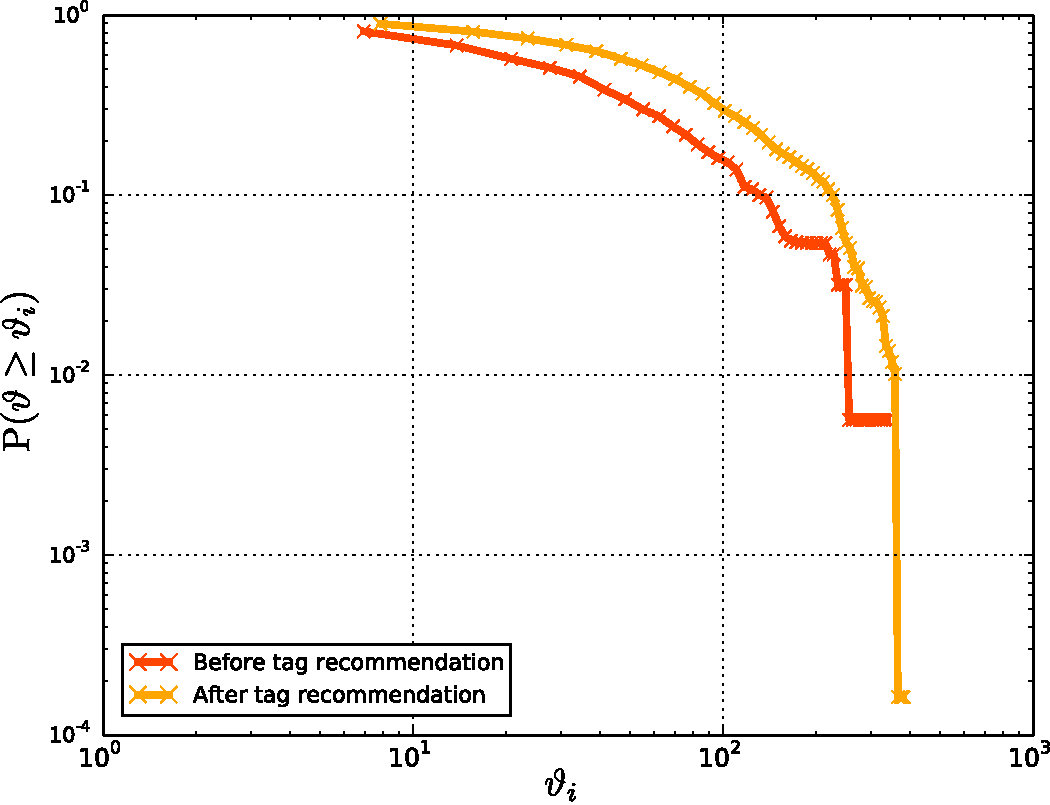
\includegraphics[width=0.66\columnwidth]{ch05_impact/pics/fig08_sounds_graph_strength}}
\caption[Complementary cumulative node strength distribution of sound-sound network]{
Complementary cumulative node strength $\nodeStrength$ distribution of sound-sound network $\soundsNetwork$ before and after the introduction of tag recommendation. Networks are build with data from analysis windows $\referenceWindowsVector_0$ and $\windowOfInterest$ respectively.}
\label{impact:fig:sounds_graph_strength}
\end{figure}


\subsubsection{Discussion}

We have seen that the tag recommendation system lessens the invention of new tags and that, at the same time, it increases the size of users' vocabulary and the number of tags that are shared among users and sounds. Thus, we can conclude that all users annotating sounds receive a common influence that positively affects the convergence of the vocabulary in the folksonomy by leveraging the reuse of tags, reducing the generation of new ones, and increasing the number of distinct tags in users' personal vocabulary.

We have also found that both user and sound vocabulary sharing are increased after the introduction of tag recommendation. This observation, combined with the increase in users' vocabulary size, leverages the value of sound annotations. It reveals a better agreement on the vocabulary of tags used to annotate sounds and also an increase of its size. Therefore, sounds are described using a more coherent and complete vocabulary.


%%%%%%%%%%%%
\subsection{Quality of annotations}
\label{impact:sec:results_quality_annotations}


\subsubsection{Average tagline length}
\label{impact:sec:length_of_tagline}

Fig.~\ref{impact:fig:length_of_tagline} shows the evolution of the average tagline length $\metricAverageTaglineLength$. We observe a clear increase after the introduction of tag recommendation. Comparing results for the analysis window $\windowOfInterest$ and reference windows $\referenceWindowsVector_m$, we observe a minimum $\metricAverageTaglineLength$ increase of 1.32 tags per sound ($\pvalue = 7.553\cdot 10^{-6}$). 
Similarly to what we noted in Sec.~\ref{impact:sec:percentage_of_new_tags_results}, Fig.~\ref{impact:fig:length_of_tagline} seems to show a global increasing tendency already before the introduction of tag recommendation. We repeated the same extra analysis of that section (i.e.,~computing the linear regression of data before the introduction of tag recommendation and correcting $\metricAverageTaglineLength$ in $\windowOfInterest$ with the linear projection of the trend) and still observed a statistically significant minimum $\metricAverageTaglineLength$ increase of 1.22 tags per sound ($\pvalue = 3.65\cdot 10^{-5}$). Considering the average tagline length for the time periods before and after the introduction of tag recommendation, the observed increase means that sounds are annotated with approximately 20\% more tags when users are influenced by the tag recommendation system. This observation is also supported by looking at the histogram of tagline lengths before and after the introduction of tag recommendation (Fig.~\ref{impact:fig:length_of_tagline_distribution}). The increase of the average tagline length suggests that annotations performed using the recommendation system are more comprehensive and, presumably, of better quality than annotations performed without the recommendation system. 

\begin{figure}
\centerline{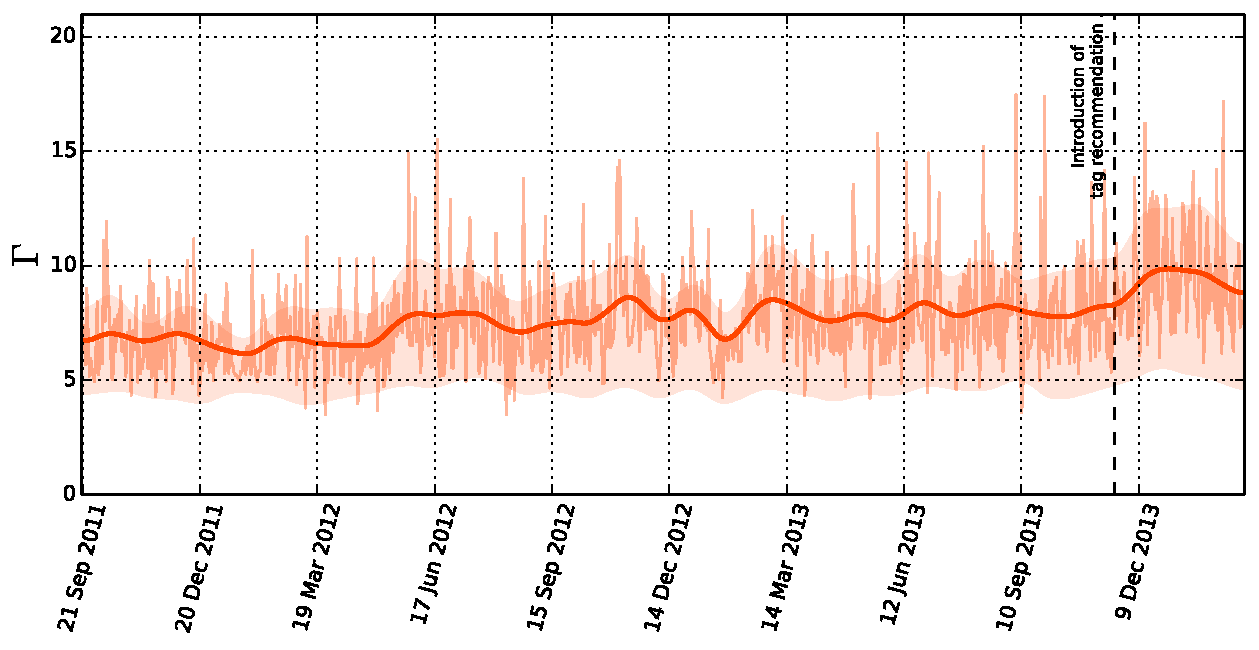
\includegraphics[width=\figSizeMax]{ch05_impact/pics/fig09_length_of_tagline}}
\caption[Evolution of average tagline length]{Evolution of average tagline length $\metricAverageTaglineLength$. The thinner line corresponds to computed $\metricAverageTaglineLength$. The bold line corresponds to a smoothed version of $\metricAverageTaglineLength$. Filled area shows the range between the lower and upper quartiles of the original data.}
\vspace{0.8cm}
\label{impact:fig:length_of_tagline}
\end{figure}

\begin{figure}
\centerline{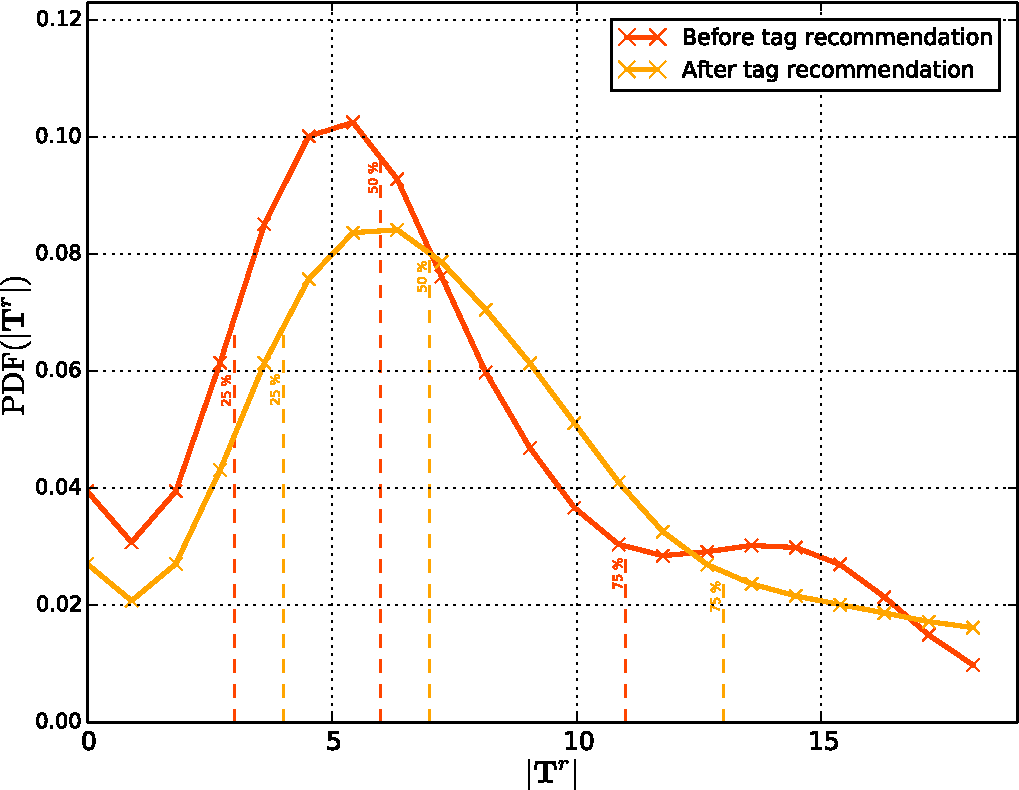
\includegraphics[width=0.7\columnwidth]{ch05_impact/pics/fig10_length_of_tagline_histogram}}
\caption[Probability density function of tagline lengths]{Probability density function of tagline lengths $|\tagsOfSoundR|$ before and after the introduction of tag recommendation. Data is drawn from the analysis windows $\referenceWindowsVector_0$ and $\windowOfInterest$, respectively. Smoothing is performed using an arbitrarily chosen Hann window of 11 points. Dashed vertical lines with attached percentage values indicate the percentage of sounds whose tagline length is less than or equal to what is indicated in the corresponding line position.}
\label{impact:fig:length_of_tagline_distribution}
\end{figure}


\subsubsection{Percentage of misspelled tag applications}
\label{impact:sec:misspelled_tag_applications}

Fig.~\ref{impact:fig:misspelled_tag_applications} shows the evolution of misspelled tag applications $\metricMispellings$. 
As expected, we observe a slight decreasing tendency in $\metricMispellings$ after the introduction of tag recommendation
When comparing results for the analysis window $\windowOfInterest$ and the other reference windows $\referenceWindowsVector_m$, we find a minimum $\metricMispellings$ decrease of 1.4\% (not statistically significant), and a maximum decrease of 5\% (statistically significant, with $p = 4.775\cdot 10^{-5}$). 
Hence, this shows that the introduction of tag recommendation has a moderate impact on misspelled tags, helping users to generate up to 5\% less tags with misspellings.

\begin{figure}
\centerline{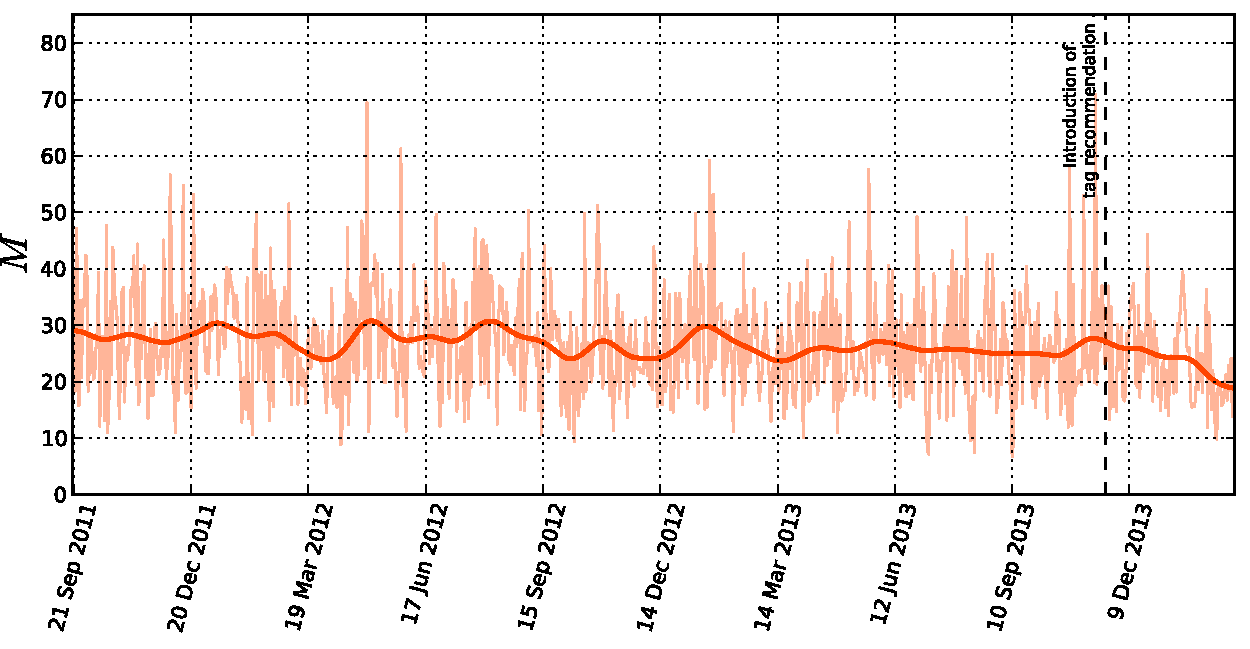
\includegraphics[width=\figSizeMax]{ch05_impact/pics/fig99_misspelled_tag_applications}}
\caption[Evolution of the percentage of misspelled tag applications]{Evolution of the percentage of misspelled tag applications $\metricMispellings$. Similarly to the previous figures, the thinner line corresponds to computed $\metricMispellings$. The bold line corresponds to a smoothed version of $\metricMispellings$.
}
\label{impact:fig:misspelled_tag_applications}
\end{figure}



\subsubsection{Tag frequency distribution} 

Fig.~\ref{impact:fig:tag_frequency_distribution} shows the complementary cumulative tag frequency distribution before and after the introduction of tag recommendation. It can be observed that the distribution after the introduction of tag recommendation tends to be more even, particularly reinforcing the usage of tags in the low and mid frequency ranges (tags with less than 800 occurrences). This means that less popular tags gain importance after the introduction of tag recommendation. Less popular tags typically correspond to narrower semantic concepts, which are used to bring more details to sound annotations. Again, this observation is consistent with previous observations regarding vocabulary convergence. It reflects an increase in both user and sound vocabulary sharing, as tags with less frequency gain importance and start being more widely used. It also suggests that annotations after the introduction of tag recommendation are more detailed as the usage of tags in the low and mid frequency ranges is reinforced.

To complement these results, we evaluated how well tag frequency distributions corresponding for the analysis windows $\referenceWindowsVector_0$ and $\windowOfInterest$ fit into a power law distribution. In both cases, the analysis shows a better fit for a log-normal distribution rather than a power law distribution. However, the tag frequency distribution after the introduction of tag recommendation shows a better fit for the power law than the distribution before tag recommendation, which may also suggest the presence of a better converging vocabulary yielding more meaningful descriptions (Sec.~\ref{impact:sec:methods_quality_of_annotations}).%\citep{Mathes2004,Cattuto2006,halpin2006,Wagner2014}.


\begin{figure}
\centerline{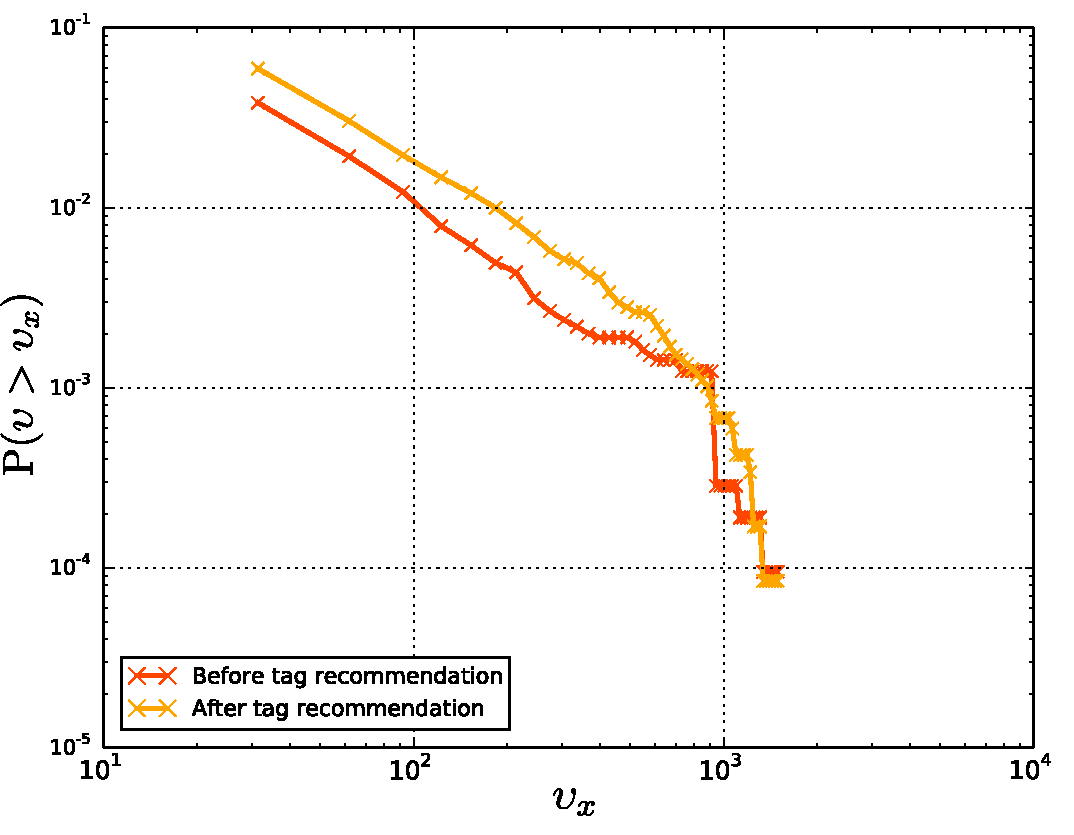
\includegraphics[width=0.7\columnwidth]{ch05_impact/pics/fig11_tag_frequency_distribution}}
\caption[Complementary cumulative tag frequency distribution]{Complementary cumulative tag frequency $\tagFrequency$ distribution before and after the introduction of tag recommendation. Data is drawn from the analysis windows $\referenceWindowsVector_0$ and $\windowOfInterest$, respectively. }
\vspace{0.8cm}
\label{impact:fig:tag_frequency_distribution}
\end{figure}


\subsubsection{Subjective annotation quality} 
We analyse the results of the online experiment described in Sec.~\ref{impact:sec:methods_quality_of_annotations} and observe a subjective annotation quality of $\metricQualitativeAnnotationQuality=0.075$ (0.81 standard deviation). One third of the quality judgements performed by the participants correspond to ``No preference'' judgements ($\unionOfQualityJudgements_j=0$). If we discard these judgements, the subjective annotation quality is increased to $\metricQualitativeAnnotationQuality=0.114$ (0.99 standard deviation), meaning that in 55\% of the judgements the sounds described using the tag recommendation system are considered to be better annotated. These results indicate that participants in the experiment have a slight tendency to consider annotations of sounds described using the tag recommendation system as being better than annotations of sounds made without the tag recommendation system.
To further validate these results, we computed Cohen's kappa coefficient to measure the agreement among the quality judgements performed by the participants in the experiment~\citep{carletta1996assessing}. 
After all possible pairwise comparisons between the different participants in the experiment, we observe an average kappa coefficient of 0.22. Thus, participants in the experiment tend to agree in their judgements. This reinforces our previous observations.

During the experiment, participants also provided textual comments about some of their quality judgements. In general, participants used comments to explain the reason why they considered sounds to be badly annotated. Among these reasons, the most common ones are the presence of misleading or uncompleted annotations, the presence of tags not related to the sound being annotated, and the presence of tags with typographical errors. In the participants' sample, all these reasons are reported evenly for sounds uploaded before and after the introduction of tag recommendation.


\subsubsection{Discussion}
We have seen that the average number of tags used to annotate a sound is larger after the introduction of tag recommendation. 
A similar observation is made in a study by~\cite{Ames2007}, in which two mobile phone applications for uploading photos to Flickr are compared. One of the applications features a tag recommendation system to aid users in the tagging process, and an increase in the average tagline length is observed for those photos uploaded with that application.

The fact that the average tagline length increases after the introduction of tag recommendation also reinforces the previously discussed observations regarding vocabulary convergence. Tag recommendation yields more tag applications and potentially more comprehensive sound annotations, and yet fewer new tags are created while vocabulary sharing is increased. Hence, our results indicate that sound annotations after the introduction of tag recommendation are done using a more coherent and complete vocabulary of tags. This fact seems to be further confirmed by the results of the online experiment we set up to analyse qualitative annotation quality, as participants on this experiment preferred annotations of sounds uploaded after the introduction of tag recommendation.

The tag frequency distribution we observe after the introduction of tag recommendation also supports the increase in the convergence of the vocabulary. 
In this case, a better agreement is reached specially for those tags with lower frequencies of occurrence. Thus, we could say that there is a better agreement on the tags users choose to annotate specific concepts, which leverages the value (and thus the quality) of the annotations.

Finally, we also observed that tag recommendation helps users in slightly reducing misspellings in the tags they introduce. This also supposes an improvement in the quality of annotations. However, the impact we observe is rather limited, which may be explained by several factors. Firstly, the way in which we estimate misspelled tags is not perfectly accurate and thus some noise is present in the metric (see Sec.~\ref{impact:sec:methods_quality_of_annotations}). Secondly, the nature of the tag recommendation system does not prevent itself from actually recommending tags with misspellings. Hence, even if it is intuitively less likely that misspelled tags will feature a strong similarity with any of the input tags, it is still possible that these are recommended. 
Finally, we can only expect tag recommendation to effectively help in reducing misspellings for the tags that are actually suggested by the system and correctly predicted. As we describe below in Sec.~\ref{impact:sec:percentage_correcly_predicted_tags_results}, approximately 19\% of the tags of a tagline are correctly predicted, and this can be taken as a rough estimate of an upper bound for the decrease in the percentage of misspelled tag applications. Furthermore, even when relevant tags are recommended by the system and are correctly predicted, many users still prefer to manually type them instead of clicking on the list of suggestions, which may still lead to misspellings (see Sec.~\ref{impact:sec:percentage_correcly_predicted_tags_results}).
That being said, overall results regarding the quality of annotations suggest that the introduction of tag recommendation has a moderate yet positive impact on this aspect.


%%%%%%%%%%%%
\subsection{Cost of the annotation process}
\label{impact:sec:cost_annotations}


\subsubsection{Average tag application time}

Fig.~\ref{impact:fig:tag_time} shows the probability density function of the average time per tag application $\metricAverageTagApplicationTime$ with and without the use of the tag recommendation system. Even though we observe a small average decrease in $\metricAverageTagApplicationTime$ for annotation sessions using the tag recommendation system, it is found to be not statistically significant ($\pvalue = 0.83$). This means that no substantial difference on the time needed to perform a tag application can be reported. However, if we look at the total amount of time invested in annotating every sound (instead of every tag), we do observe a statistically significant average increase of roughly 35 seconds per sound after the introduction of tag recommendations ($\pvalue = 6.2\cdot 10^{-3}$), which represents an increase of approximately 20\%. This is consistent with the 20\% increase of the tagline length we observed in Sec.~\ref{impact:sec:length_of_tagline}. Thus, in general, we could say that users need at least the same amount of time to perform a single tag application as they needed before using the system. However, annotations are longer and therefore users spend more time annotating sounds.

\begin{figure}
\centerline{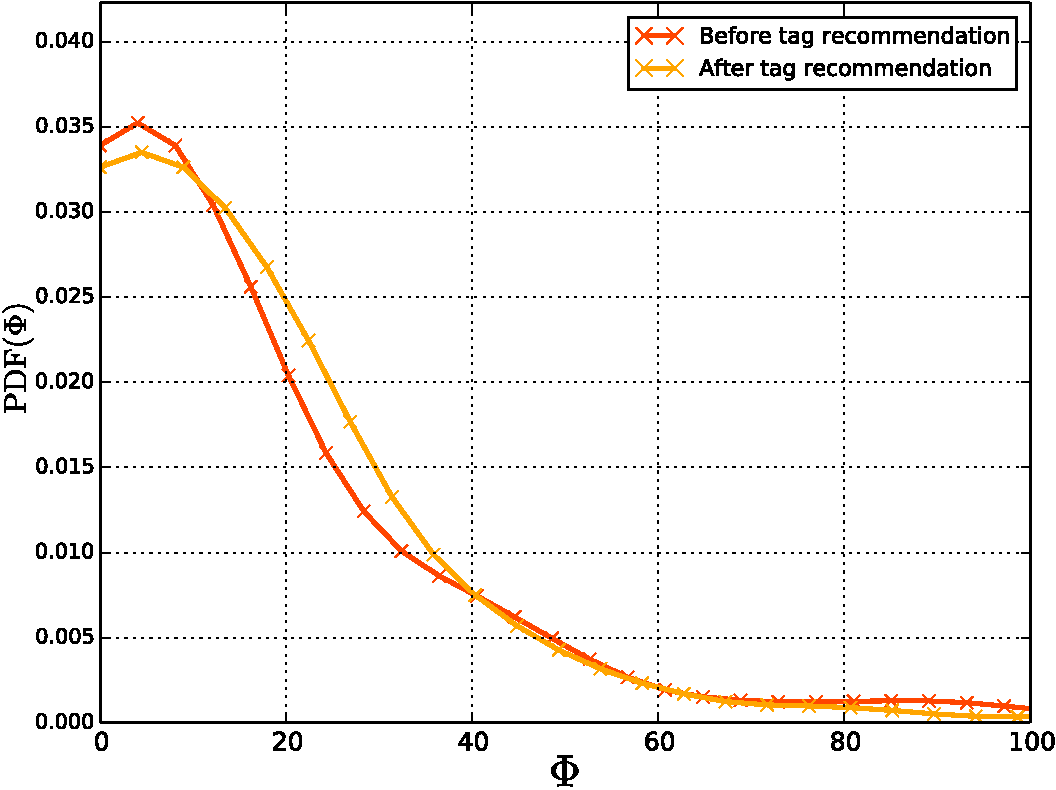
\includegraphics[width=0.7\columnwidth]{ch05_impact/pics/fig12_time_pdf}}
\caption[Probability density function of the average tag application time]{Probability density function of the average tag application time $\metricAverageTagApplicationTime$ with and without the tag recommendation system. Curves are smoothed using a Hann window of 11 points.}
\label{impact:fig:tag_time}
\end{figure}


\subsubsection{Average number of correctly predicted tags}
\label{impact:sec:percentage_correcly_predicted_tags_results}

As explained in Sec.~\ref{impact:sec:definition_of_metrics}, the average number of correctly predicted tags $\metricPercentageOfCorrectlyPredictedTags$ can only be computed with data drawn from $\windowOfInterest$. Computing it on a daily basis shows that an average of 2.10 tags (from those finally assigned to sounds) were suggested by the recommendation system. This corresponds to approximately 19\% of tags in a tagline. This is similar to what we found in Chapter~\ref{sec:class} (Table ~\ref{tab:results_general_ub}), in which an average of 2.41 tags were correctly predicted by the class-based tag recommendation method (corresponding to approximately 29\% of the tags in a tagline). 
%The bigger difference between both numbers of correctly predicted tags when expressed as a percentage can be explained because the average tagline length was lower in the experiment performed in Chapter~\ref{sec:class} as compared to the current experiment.%7.4
Hence, according to these results, the tag recommendation system behaves similarly both in the real-world and in a controlled environment, with a certain tendency of users accepting fewer tags in the real world.

Among the correctly predicted tags, we make a distinction between those that are added to the tagline by users clicking on the corresponding tag in the list of suggestions, and those that are manually typed by users. If we only consider the tags that are added to the tagline by users actively clicking on the suggestion, we observe an average number of 1.58 correctly predicted tags, corresponding to approximately 13\% of the tags in a tagline. This suggests that, in many occasions, users still prefer to manually type the tags instead of switching to the mouse and clicking on the list of suggestions.
In general, these results show that, even though an important part of the final tagline for a sound can be constructed using tags suggested by the recommendation system, the majority of these tags have to be generated by users themselves, and are not necessarily related with those suggested by the system.
%This also partially explains why the impact on the average time per tag application we reported above is rather minimal, although in any case it is not clear whether the act of clicking on the list of suggestions would require less time than manually typing the tag.


\subsubsection{Discussion}
\label{impact:sec:cost_annotation_process_discussion}
Contrary to what we expected, we have observed that the tag recommendation system does not seem to have a significant impact on the cost of the annotation process. 
Although we have seen that users need significantly more time to annotate individual sounds when using the tag recommendation system, we have also seen that this increase can be attributed to the proportional increase of the average tagline length. Hence, the actual time required for every individual tag application does not significantly change.
Furthermore, we observed that most of the tags assigned to sounds are not drawn from the list of recommended tags, meaning that most of the annotation process still consists of a generation process where users create tags from scratch rather than a recognition process where users validate tags from a list of suggestions.
 
There are several potential reasons why we do not observe the expected impact on the cost of the annotation process.
On the one hand, we observed that only 13\% of the tags in taglines are added from the list of suggestions by actually clicking on them. Hence, assuming that it is faster to click on tags rather than to manually type them (which is probably not always true), the impact we can expect on the time required for introducing tags should be lower than that 13\%.
Also, it seems intuitively plausible that users need more time to generate the tags (or recognise them from a list) than to actually introduce them. Hence, the potential impact of lessening the time required for introducing tags is further reduced.
On the other hand, the impact of the recommendation system is again limited by the fact that most of the introduced tags are not drawn from system recommendations, and thus an important part of the annotation process does not significantly change after the introduction of tag recommendation. In fact, our results might be suggesting that the cost of the recognition process is not actually lower than the cost of the generation process. This also seems reasonable, as the union of all recommended tags for a given sound is much larger than the length of the actual tagline (i.e., new tags are recommended every time that a tag is added to the tagline, see Sec.~\ref{impact:sec:tag_rec_interface}). Therefore, the recognition process must operate over a large set of tags. 

Finally, we believe that our metrics regarding the cost of the annotation process are highly dependent on the particular interface of the recommendation system. Also, the recommendation interface can have different impacts according to how users adapt to it.
Unfortunately, our analysis does not contain data to be compared coming from other recommendation interfaces. 
However, to get some more insight into that aspect, we repeated the calculations of the average tag application time but this time considering experienced and non-experienced users separately. We divided users according to the number of sounds they uploaded during our analysis period. In particular, we set the threshold at the third quartile of the distribution of uploaded sounds per user, which corresponds to 7 uploaded sounds. What we observe is that the average tag application time after the introduction of tag recommendation increases for non-experienced users and decreases for experienced users by a similar amount of about 3 seconds per tag application ($p = 2.15\cdot 10^{-3}$ and $p = 3.65\cdot 10^{-3}$, respectively). 
This shows that experienced users were able to take advantage of the recommendation interface and generate annotations slightly faster, but it also shows that the interface had a negative impact on non-experienced users, apparently increasing the cost of the annotation process.
This could be explained because experienced users probably have a better understanding of the tagging process and can easily interpret and take advantage of tag recommendation.
Nevertheless, we think that to draw more consistent conclusions regarding the impact of tag recommendation on the cost of the annotation process, further research should be carried out.


%%%%%%%%%%%%%%%%%%%%%%%%%%%%%%%%%%%%%%%%%%%%%%%%%%%%%%%%%%%%%%%%%%%%%%%%%%%%%%%%%%%%%%%%%%%%%%%%%%%%%%%%%%%%%

\section{Conclusion}
\label{impact:sec:conclusion}

In this chapter we have analysed the impact of a state of the art tag recommendation system into the real-world folksonomy of a large-scale sound sharing platform, Freesound. After a the review of current related work done in Chapter~\ref{sec:SOA} (Sec.~\ref{sec:soa:impact_tag_recommendation}), we have identified three main hypotheses regarding the impact that such a system should have when introduced into a tagging system, and we have defined several reusable metrics to evaluate that impact. We have analysed data comprising of a period from 21 September 2011 to 28 February 2014, the last three months of which correspond to data after the introduction of tag recommendation. To the best of our knowledge, these kind of quantitative analyses have not been done before using large-scale data from a real-world folksonomy. Hence, no empirical assessment of the three identified hypotheses was available to date. %The definition of several necessary metrics to assess the three hypotheses is also a further contribution of this chapter.

Our results show a significant impact of tag recommendation into most of the metrics we defined. However, the result of a single metric in isolation is probably not entirely relevant in our analysis. Instead, the fact that we observe how the changes on several metrics can be explained by some of the outlined hypotheses gives a particular value to our analysis. Overall we observe that the first hypothesis (regarding vocabulary convergence) is clearly validated, that the second one (regarding the quality of annotations) only seems to be partially validated, and the third one (regarding the cost of the annotation process) does not seem to be validated.  However, we believe the latter is particularly dependent on the annotation interface, and that its impact could be greatly improved by designing an interface specifically focused on reducing the cost of the annotation process.

Although in this work we only analyse data in the context of Freesound, we believe that our results are, to some extent, indicative of the impact that tag recommendation can potentially have in other tagging systems.
However, tagging systems of different nature may react differently to the introduction of a tag recommendation system.
An important aspect here is to take into account the motivations that users have for tagging their resources.
In narrow folksonomies such as Freesound and Flickr, users typically tag their content so that other users (and also themselves) can easily find it in the future. However, resources are only annotated once, and therefore the tags added by the uploader of a resource should also be meaningful to other users of the platform. Contrarily, in broad folksonomies such as Delicious and CiteULike, resources are tagged multiple times by several users, and thus the main motivation for tagging is users' self organisation of the content, without necessarily considering the global context of the sharing platform (Secs.~\ref{soa:user_motivations} and~\ref{soa:types_of_tags}). 
As a result, very different tagging styles can arise because of the particularities of these two kinds of tagging systems.
The tag recommendation system that we use here is designed for narrow folksonomies. It does not try to personalise recommendations to particular users' tagging behaviours, but instead it learns from parts of the folksonomy on the basis of five audio classes (Sec.~\ref{class:sec:class_based_tag_rec_ref}).
Hence, we expect it to have a bigger impact in tagging systems featuring narrow folksonomies, where the more uniform across users a tagging style is, the better the platform becomes in providing content to other users.

Importantly, the metrics and analysis methodology described here are applicable to other collaborative platforms either featuring broad or narrow folksonomies. To further assess the validity of our results, an analysis with data coming from other tagging systems and tag recommendation systems should be performed. The main obstacle for carrying out this analysis is the limited availability of comprehensive tagging data, including annotations performed \emph{with} and \emph{without} the use of a tag recommendation system, and that comprise user activity for as long a period of time as the the one we analysed.

There are several aspects of the data we already collected that could be further researched to gain more insight into the impact of the tag recommendation system. 
Firstly, we do not perform any study of the generated taglines at the semantic level. By applying techniques for mapping tags to semantic concepts or categories~\citep[e.g.,][]{cantador2010}, we could analyse the impact of the recommendation system at the semantic level, and see if it effectively shapes tagging behaviour to a more extensive usage of particular kinds of tags such as content-related or self-organisational tags. Similarly, it could be further studied if other typical problems of tagging systems such as synonymy or polysemy are in fact affected by the use of a recommendation system.
Secondly, in the current work we just introduced the concept of user experience when analysing our results in Sec.~\ref{impact:sec:cost_annotation_process_discussion}. It would be interesting to further investigate this aspect by analysing the impact of the recommendation system to other evaluation metrics when considering users with different levels of expertise.
Thirdly, another way in which the current analysis could be further developed would be with the use of network analysis techniques to inspect the user-user and sound-sound networks built on the basis of shared tags. Using such analysis, it would be interesting to evaluate the existence of community structure in those networks and to see how potential communities in both networks might be related. For example, we could investigate if there are strongly connected communities of users that annotate sounds with a particular tagging style, and then see how the introduction of tag recommendation would affect those communities.

In our opinion, the biggest future challenge in tag recommendation is the design of systems that have a bigger impact on the quality of annotations. Annotations are very subjective and difficult to evaluate. However, a recommendation system could be designed to particularly focus on that issue by driving recommendations at higher semantic levels, for example being able to select candidate tags for recommendation in terms of variety and coverage of different semantic facets. 
In order for tag recommendation systems to have a deeper impact in the tagging behaviour and in the quality of annotations, we probably need to evolve the basic tag recommendation methods into \emph{assistive} processes where we can better guide users during the annotation process. % by having more knowledge about the semantics of our tags and the particular domain we are recommending tags for. 
%We foresee that one interesting research direction is the use of ontologies to drive future tag recommendation/assistive tagging systems. Such ontologies should embed knowledge about the domain for which we are recommending tags, including relations between tags and even organising tags into different categories regarding the kind of semantic information they are describing about the resources being annotated.
In the following chapter (Chapter~\ref{sec:ontology}), we explore this perspective by proposing an extension of the current class-based tag recommendation method which takes advantage of a domain-specific ontology to drive the recommendation process.


